%%%%%%%%%%%%%%%%%%%%%%%%%%%%%%%%%%%%%%%%%%%%%%%%%%%%%%%%%%%%%%%%%%%%%%%%%%%%%%%%
%2345678901234567890123456789012345678901234567890123456789012345678901234567890
%        1         2         3         4         5         6         7         8

\documentclass[letterpaper, 10 pt, conference]{IEEEtran}  % Comment this line out
                                                          % if you need a4paper
%\documentclass[a4paper, 10pt, conference]{ieeeconf}      % Use this line for a4
                                                          % paper

\IEEEoverridecommandlockouts                              % This command is only
                                                          % needed if you want to
                                                          % use the \thanks command
\overrideIEEEmargins

%US Letter first page 	Top 1 Left 0.75 Right 0.75 Bottom 0.75 in
%US Letter other pages 	Top 0.75 Left 0.75 Right 0.75 Bottom 0.75 in
\usepackage[top=1in, bottom=0.75in, left=0.75in, right=0.75in]{geometry}
\usepackage{times}
%\usepackage[T1]{fontenc}
%\usepackage{tikz}
\usepackage{amsmath}
%\usepackage{amsthm}
%\usepackage{verbatim}
\usepackage{subfigure}
\usepackage{graphicx}
\usepackage{wrapfig}
%\usepackage{geometry}

\newcommand{\comments}[1]{}
% See the \addtolength command later in the file to balance the column lengths
% on the last page of the document



% The following packages can be found on http:\\www.ctan.org
\usepackage{graphics} % for pdf, bitmapped graphics files
\usepackage{epsfig} % for postscript graphics files
\usepackage{mathptmx} % assumes new font selection scheme installed
\usepackage{times} % assumes new font selection scheme installed
\usepackage{amsmath} % assumes amsmath package installed
\usepackage{amssymb}  % assumes amsmath package installed

\usepackage{amsmath}
\interdisplaylinepenalty=2500

\title{\LARGE \bf
The Conjugate Unscented Transform - An Approach to Evaluate Multi-Dimensional Expectation Integrals
}

%\author{ \parbox{3 in}{\centering Nagavenkat Adurthi*
%         \thanks{*Use the $\backslash$ graduate student}\\
%         MAE Department \\
%         University of Twente\\
%         7500 AE Enschede, The Netherlands\\
%         {\tt\small h.kwakernaak@autsubmit.com}}
%         \hspace*{ 0.5 in}
%         \parbox{3 in}{ \centering Pradeep Misra**
%         \thanks{**The footnote marks may be inserted manually}\\
%        Department of Electrical Engineering \\
%         Wright State University\\
%         Dayton, OH 45435, USA\\
%         {\tt\small pmisra@cs.wright.edu}}
%}

\author{\begin{tabular}{cccc}
 Nagavenkat Adurthi  &  Puneet Singla &  Tarunraj Singh \\
\small Graduate Student & \small Assistant Professor &\small Professor \\
\small nagavenk@buffalo.edu & \small psingla@buffalo.edu & \small tsingh@buffalo.edu %\vspace{0.01in}
\end{tabular}\\
%\textsl{Department of Mechanical \& Aerospace Engineering}\\
\textsl{University at Buffalo, The State University of New York,
Amherst, NY 14260-4400}}

\begin{document}



\maketitle

\thispagestyle{empty}
\pagestyle{empty}


%%%%%%%%%%%%%%%%%%%%%%%%%%%%%%%%%%%%%%%%%%%%%%%%%%%%%%%%%%%%%%%%%%%%%%%%%%%%%%%%
\begin{abstract}
This paper presents an extension to the unscented transformation to evaluate expectation integrals in general $N$-dimensional space by satisfying higher order moment equations. New sets of sigma points are defined to satisfy moment equations up to order  $8$.  The proposed methodology can be used as an efficient alternative to Gaussian quadrature rule with significantly reduced number of function evaluations but without any loss in accuracy. The proposed methodology is compared to the Gauss Hermite product rule and many other computational algorithms by considering benchmark problems. Numerical simulation results illustrates the effectiveness of the proposed methodology in computing high dimension expectation integrals with significantly reduced number of function evaluations.\end{abstract}


%%%%%%%%%%%%%%%%%%%%%%%%%%%%%%%%%%%%%%%%%%%%%%%%%%%%%%%%%%%%%%%%%%%%%%%%%%%%%%%%
\section{INTRODUCTION}

Numerous fields of science and engineering present the problem of uncertainty characterization and propagation through nonlinear dynamic systems with stochastic excitation and uncertain initial conditions. One may be interested in predicting the probability of collision of asteroid with Earth, diffusion of toxic materials through atmosphere, control of movement and planning of actions of autonomous systems, the optimization of financial investment policies, or simply the computation of the prediction step in the design of a Bayes filter. All these applications require the study of the relevant stochastic system and involve computing multi-dimensional expected value integrals involving appropriate probability density function (pdf). Analytical expressions for these multi-dimension integrals exist only for linear systems and only for few moments. For example, the well celebrated Kalman filter provides the analytical expressions for mean and covariance of linear system subject to Gaussian white noise and Gaussian initial condition errors. However, one often do not have direct analytical solution for these integrals and have to approximate integral values by making use of computational methods.

Several computation techniques exist in the literature to approximate the expectation integral values, the most popular being Monte Carlo (MC) methods, Gaussian Quadrature Rule, Unscented Transformation (UT) and Cubature methods. All these methods involve an approximation of the expectation integral as a weighted sum of integrand values at specified points within the domain of integration. These methods basically differ from each other in the generation of these specific points. For example, MC methods involves random samples from the specified pdf while Gaussian quadrature scheme involves deterministic points carefully chosen to reproduce exactly the integrals involving polynomial functions. Both deterministic Gaussian quadrature and MC methods are very popular but both methods require extensive computational resources and effort, and becomes increasingly infeasible for computing expectation integrals in high-dimension space~\cite{strGQF}. 

For one-dimensional integrals, one needs $m$ quadrature points according to the Gaussian quadrature scheme to reproduce the expectation integrals involving $2m-1$ degree polynomial functions. However, for a generic $N$-dimensional system, one needs to take the tensor product of $1-$dimensional $m$ quadrature points and hence one would require a total of $m^N$ quadrature points (also known as cubature points for $N\ge2$)~\cite{strGQF}.  Even for a moderate dimension system involving $6$ random variables, the number of points required to evaluate the expectation integral with only $5$ points along each direction is $5^6=15,625$. This is a huge number of points that might be computationally expensive to use especially when the evaluation of function at each cubature point itself can be an expensive procedure.%, e.g., one may need to solve a system of partial differential equations to compute the function of interest. 
But fortunately the Gaussian quadrature rule is \emph{not minimal} for $N\ge2$ and there exists cubature rules with reduced number of points~\cite{strGQF}. This forms the basis of our motivation to the work presented in this paper.

An extensive amount of work has been done in this field to develop cubature/quadrature rules which can exactly reproduce integrals involving polynomials of degree less than or equal to `$d=2m-1$'   with fewer points, i.e.,  less than $m^N$.  A good description of non-product Gaussian cubature rules, particularly for symmetric density functions, that are second, third and fifth degree exact in any dimension is provided in ~\cite{strACMI}. In general to develop a cubature rule of degree `$d$' that is applicable to any dimension is still an open problem. A cubature rule of degree 2 with $N+1$ points and a cubature method of degree 3 with $2N$ points for a general centrally symmetric weight function (such as the normal and uniform pdf) in $N$-dimensions is developed in ~\cite{str2d}. A fully symmetric integration rules with minimal points for $2$-dimension are developed that are exact for degree $9-15$ in ~\cite{phil2D}.  A $19$ point cubature rule is developed, for symmetric regions in 2-dimensions that are exact for degree 9 or less in ~\cite{Robd92D}. For a $2$-dimensional integral, with symmetric weight function a $12$ point cubature rule for degree $7$  is developed in \cite{Richd72D}. It is even claimed that this is the minimal number of points required and there exist many such 12 point cubature rule for degree
\newgeometry{top=0.75in,right=0.75in,left=0.75in,bottom=0.75in} 
  $7$ in $2$-dimensional systems. %In the perspective of filtering where the integrals with normal probability density functions arise, the cubature methods with reduced number of points have known to be a very useful. 
The highly acclaimed Unscented Transform (UT) with only $2N+1$ points is a degree $3$ cubature method, where these cubature points are now called \emph{sigma points}~\cite{jul1}. Similar to the UT method, a more recent development is the Cubature Kalman filter (CKF) which is again exact to degree 3 but uses only $2N$ points~\cite{Arackf}. It is to be mentioned that the sigma/cubature points of $2N+1$ UT and $2N$ CKF, though they have different elegant approaches, are infact \emph{special cases} of a more general work previously done in~\cite{str2d} for any symmetrical probability distribution function.  

Most of the non-product cubature rule possess certain similarities, they exploit the symmetry of the weight function, assume a structure for the cubature points, solve a system of nonlinear equations. Hence these methods also suffer some similar drawbacks such as inconsistency of the set of nonlinear equations, the presence of negative weights/complex roots and the inability to provide a generalized solution that works for any dimension. The present work heads in a similar manner and tries to overcome some of these difficulties. 

 The primary objective of this paper can be stated as "To find a fully symmetric sigma/cubature point set with all positive weights and reduced number of points that is \emph{equivalent} to the set of cubature points of Gaussian quadrature product rule of \emph{same order}". \emph{Equivalent to same order} implies that for a polynomial of order $2m-1$ in generic $N$-dimensions, both the new reduced sigma point set from the proposed method known as Conjugate Unscented Transform method (`CUT') and the $m^N$ quadrature points from the Gaussian quadrature product rule result in same order of relative percentage error. The organization of paper is as follows: firstly, we review few popular cubature rules, particularly the Unscented Transfrom. A intuitive understanding of how these methods tend to pick the sigma/cubature points provides a valuable insight upon which our development of the framework/methodology for the Conjugate Unscented Transfrom is based. Secondly, we describe this framework/methodology to evaluate the sigma point sets for the three methods we intend to propose along with numerical results to show the efficacy of each method compared to Gauss Hermite Product rule. 
%%%%%%%%%%%%%%%%%%%%%%%%%%%%%%%%%%%%%%%%%%%%%%%%%%%%%%%%%%%%%%%%%%%
   %%%%  Importance of Higher-Order Moments  %%%%%%%%
%%%%%%%%%%%%%%%%%%%%%%%%%%%%%%%%%%%%%%%%%%%%%%%%%%%%%%%%%%%%%%%%%%%

\section{Expectation Integral and Cubature Methods}
Let us consider the problem of computing expected value of a function $f(x)$ with respect to a Gaussian density function. Without loss of generality consider the mean and covarince of the Gaussian function to be zero and unity, respectively. % with zero mean $and covariance $P$: 
\begin{align}
E[f(x)]&= \int{f(x)N(x,0|1)}dx \label{exptint}
\end{align}
Taking the Taylor series expansion of $f(x)$ about the mean and substituting in the aforementioned expression leads to
\begin{align}
E[f(x)]&= f(0)+\nabla{f(0)}E[{x}]+\frac{1}{2!}\nabla^2f(0)E[{x}^2]\nonumber \\ 
&{+}\: \frac{1}{3!}\nabla^3f(0)E[{x}^3]+\frac{1}{4!}\nabla^4f(0)E[{x}^4]... \label{exptinttaylor}
\end{align}
Notice that the problem of evaluating the expected value of nonlinear function $f(x)$ has reduced to computing higher order moments of $x$. Thus by increasing the number of terms in the Taylor series expansion, one can obtain more accurate value of the expectation integral of \eqref{exptint}. Furthermore, consider the discrete approximation of \eqref{exptint} as a weighted average of  $f(x)$ evaluated at each quadrature/sigma point set $(x_1,x_2,...,x_n)$ with corresponding weights $(w_1,w_2,...w_3)$:
\begin{align}
E[f(x)]&{}\approx\sum_{i=1}^n{w_if(x_i)}\label{sigmasum}
\end{align}
Now, substitution of the Taylor series expansion about the mean for $f(x_i)$ in \eqref{sigmasum} leads to: %Consider the Taylor series approximation of the function value at each point about the mean as in (\ref{sigmataylor})
%\setlength{\arraycolsep}{0.0em}
%\begin{eqnarray}
%f(x_i)&{}={}& f(0)+\frac{1}{2!}\nabla^2f(0)x_i^2\nonumber \\ 
%&&{+}\: \frac{1}{4!}\nabla^4f(0)x_i^4+\frac{1}{6!}\nabla^6f(0)x_i^6... \label{sigmataylor}
%\end{eqnarray}
%\setlength{\arraycolsep}{5pt}
% which on substituting into (\ref{sigmasum}) results in (\ref{compeqnssigtotay}) that is in terms of the sigma points and associated weights. 
% \setlength{\arraycolsep}{0.0em}
\begin{align}
E[f(x)]&{}={} f(0)(\sum_{i=1}^n{w_i})+\frac{1}{2!}\nabla^2f(0)(\sum_{i=1}^n{w_ix_i^2})\nonumber\\
&{+}\: \frac{1}{4!}\nabla^4f(0)(\sum_{i=1}^n{w_ix_i^4})+\frac{1}{6!}\nabla^6f(0)(\sum_{i=1}^n{w_ix_i^6}) \label{compeqnssigtotay}
\end{align}
 Comparing the coefficients of $f(0)$ and derivatives of $f(x)$ evaluated at $0$ from \eqref{compeqnssigtotay} and \eqref{exptinttaylor} leads to the following set of equations known as the \textit{moment constraint equations:} 
\begin{align}
\sum_{i=1}^n{w_ix_i^m}&{}={}E[{x}^m], \quad  m=0,1,2,\cdots \label{momentconst}
\end{align}
Notice that these constraint equations simply  conveys that the sigma points $x_i$ should satisfy the infinite moment equations in the domain of the pdf, i.e., $x$-space. Thus, if $f(x)$ is a polynomial function of degree $d$ then sigma points should be chosen to reproduce first $d$ moments of the pdf exactly to guarantee the exact evaluation of the expectation integral of \eqref{exptint}. For non-polynomial functions, one have to judiciously choose the number of moment equations which should be satisfied. These one-dimensional moment constraint equations can easily be generalized for generic $N$-dimensional system as illustrated in \cite{jul1}. 
For example, Table~\ref{moment_match} shows all the moment equations till $4^{th}$ order moment in two dimensions.
\begin{table}
\caption{Moment Constraint equations for 2D till order 4}\vspace{-0.15in}
\label{moment_match}
\begin{center}
\begin{tabular}{|c|c||c|c|}
\hline
Continuous & Discrete & Continuous & Dicrete\\
\hline
$E[x]$ & $\sum_{i=1}^n{w_ix_i}$& $E[y]$ & $\sum_{i=1}^n{w_iy_i}$\\
\hline
$E[x^2]$ & $\sum_{i=1}^n{w_ix_i^2}$& $E[xy]$ & $\sum_{i=1}^n{w_ix_iy_i}$\\
\hline
$E[y^2]$ & $\sum_{i=1}^n{w_iy_i^2}$& $E[x^4]$ & $\sum_{i=1}^n{w_ix_i^4}$ \\
\hline
$E[y^4]$ & $\sum_{i=1}^n{w_iy_i^4}$& $E[x^3y]$ & $\sum_{i=1}^n{w_ix_i^3y_i}$\\
\hline
$E[y^3x]$ & $\sum_{i=1}^n{w_iy_i^3x_i}$ & $E[x^2y^2]$ & $\sum_{i=1}^n{w_ix_i^2y_i^2}$\\
\hline
\end{tabular}
\end{center}\vspace{-0.2in}
\end{table}

As discussed in the last section, one intends to seek a set of sigma points that satisfy all the moment constraint equations till the prescribed order $d$.  Many computational methods have been discussed in literature to choose a set of points which satisfy the moment equations up to a desired order with Gaussian quadrature methods being most popular. Although Gaussian quadrature methods can be generalized to satisfy these moment equations to a prescribed order $d$, these methods suffer from \textit{curse of dimensionality} with number of points increasing exponentially with increase in dimension. As an alternative to Gaussian quadrature scheme, many non-product methods~\cite{str2d,phil2D,Robd92D,Richd72D,jul1,Arackf,str5d} and \cite{str7d} have been discussed in literature to seek minimal number of sigma points to satisfy the desired number of moment equations. However, the development of a cubature rule of degree `$d$' that is applicable to any dimension is still an open problem.% Recently, Julier et al.~\cite{jul1} present a cubature method known as Unscented Transformation which guarantee the satisfaction of moment equations up to degree 2 with $2N+1$ points for the evaluation of generic $N$-dimensional expectation integrals involving Gaussian pdf. It should be mentioned that similar method is presented in \cite{strACMI} for the evaluation of expectation integrals jul1 uniform pdf $2N$ points which guarantees the satisfaction of the moment equations up to degree 2. 
The main purpose of this work is to extend the effort of few previous non-product rules, particularly the conventional unscented transformation to compute the expectation integrals involving Gaussian pdf  while satisfying the higher order moment equations.  

\section{Unscented Transformation}
In this section, we briefly discuss the main idea of the conventional UT. The conventional UT algorithm involves the selection of $2N+1$ sigma points such that first two moment equations are satisfied~\cite{jul1}. For a zero mean and unity covariance, these sigma points are chosen such that one of the point lies at the origin and the remaining $2N$ points are constrained to lie symmetrically about the mean on $N$-orthogonal axes, known as principal axes, at a distance $r_1$. The variable $r_1$ is chosen to be $\sqrt{N+\kappa}$  such that the second order moment equations are satisfied and an analytical expression for sigma point weights can be obtained. 
\begin{align}
X_0&=\mu  &W_0&={\kappa}/{(N+\kappa)}\label{UTw0}\\
X_i&=\mu+(\sqrt{(N+\kappa)P})_i  &W_i&={1}/{[2(N+\kappa)]} \label{UTw1}\\
X_{i+N}&=\mu-(\sqrt{(N+\kappa)P})_i 	 &W_{i+N}&={1}/{[2(N+\kappa)]}\label{UTw2}
\end{align}
%With $\mu=\vec{0}_{(N\times 1)}$ and $P=I_{(N\times N)}$, by an elegant selection of $r_1=\sqrt{N+\kappa}$ one could solve for $w_1$ from (\ref{str2ndmom}), $w_0$ from (\ref{centwt2ndequi}) and $\kappa$ from (\ref{str4thmom}) as
% \setlength{\arraycolsep}{0.0em}
%\begin{align}
%w_1&={1}/{2(N+\kappa)}\\
%w_0&=1-2Nw_1={\kappa}/{(N+\kappa)}\\
%N&+\kappa =3
%\end{align}
%\setlength{\arraycolsep}{5pt}
where $i$ varies from $1$ to $N$. It should be mentioned that the principal axes for the generation of sigma points correspond to each column of the identity covariance matrix or the square root of the covariance matrix in general. To find the sigma points of an arbitrary Normal pdf, one can always find the sigma points with respect to a normal pdf with zero mean and unity covariance and then apply \emph{affine transformations} to each point. A description of such affine transformations can be found in \cite{strACMI,Arackf}.   
%It is defined as the orthogonal axis in cartesian space intersecting at the origin. These are the axis corresponding to each column of the identity covariance matrix. Thus there are $N$ principal axis or $2N$ distinct points on the principal axis for N-Dimensional system. Let the set $D=\{1,2,3,...,N\}$  We list the points on the principal axis as 
%%\setlength{\arraycolsep}{0.0em}
%\begin{equation}
%\sigma_i \in \{\pm(I)_j|j\in D\} \quad i=1,2,3,...,2N.
%\end{equation}
%Each point on the principle axis is at a distance $|\sigma_i|$ or in this case at 1 unit distance from the origin, where $|x|=\sqrt{x_1^2+x_2^2\cdots x_N^2}$. The principle axis labeled as $\sigma$ and the corresponding points are shown for a 2D case in Fig(\ref{fig:allaxissubfig1}) while for a 3D case only one of the quadrant is shown in two perspective views as Fig(\ref{fig:allaxissubfig2}) and Fig(\ref{fig:allaxissubfig3}). All the 8 quadrants in the 3D case are symmetrical.
Furthermore, the tuning parameter $\kappa$ is generally chosen such that one of the $4^{th}$ moment equation error can be minimized which leads to the constraint of $N+\kappa=3$. % on the value of $\kappa$:
%\begin{equation}
%N+\kappa=3
%\end{equation}
This methodology works well for systems till dimension 3 after which the weight corresponding to the central point becomes negative, which can lead to indefinite covariance matrix. 

Tenne et al.~\cite{dirk} have developed higher order unscented transformation method for a general pdf in one dimensional system which can satisfy the moment equations up to $8^{th}$ order. L\'{e}vesque generalizes the method presented in \cite{dirk} to develop unscented transformation for generic $N$-dimension system~\cite{leves}. However, this method fails to capture cross moments. 
It is clear that obtaining $4^{th}$ order accurate sigma points for higher dimensions is still a challenge. One has to note that most of the non-product rules tend to judiciously select a specific structure of the points. Conventional UT and CKF methods are based upon the fact that constraining the points to lie on principal axis leads to \emph{the minimal number of points} required to satisfy moment equations up to order 2.


%For example, the methods of $2N+1$ UT and $2N$ CKF \emph{assume} the points to lie on the principle axis. One could easily choose a different symmetric set of axis to constrain the points in order to satisfy the $2^{nd}$ moment equations. But it so happens that the clever choice of constraining points to the principle axis leads to \emph{the minimal number of points}. % generalize the method of  Tanne et al. to develop unscented transformation for generic $N$-dimension system. However, this method does not capture the cross moments like ????. 

In summary, the set of nonlinear moment constraint equations are very tedious to solve for a general $N$-dimensional system. The UT provides an insight that ``the points can be constrained to some \emph{carefully} selected axis'' and one needs to solve for only the distances of these points from the origin and their corresponding weights. One has to be judicious in the selection of appropriate axis. The set of moment constraint equations along with these additional constraints makes the system easier to solve. However, choosing an appropriate axis is not a \emph{trivial} problem. 

Let us consider the problem of selecting sigma points such that first four moment equations are satisfied. Assuming i.i.d random variables $(X_1,X_2,\cdots,X_N)$ with zero mean and identity covariance lead to following higher order moments till order 4:
\begin{align}
E[X_i^2]&=1, &E[X_iX_j]&=0,  &E[X_i^4]&=3 \nonumber\\
E[X_i^3X_j]&=0, &E[X_i^2X_j^2]&=1, &E[X_i^2X_jX_k]&=0 \nonumber\\
E[X_iX_jX_kX_l]&=0,& & & &\label{4thmoms}
\end{align}
Where $\{i,j,k,l\}\subset\{1,2,3,...,N\}$. Like in the conventional UT scheme, a fully symmetric set of sigma points that lie on the principal axis such that the distance of each point from the origin $r_1$ and each has weight of $w_1$ leads to following constraint equations:
\begin{align}
E[X_i^2]     &\equiv 2r_1^2w_1=1 \label{str2ndmom}\\
E[X_i^4]     &\equiv 2r_1^4w_1=3 \label{str4thmom}\\
E[X_i^2X_j^2]&\equiv       0  \neq1 \label{cross4thmom}\\
1=&w_0+2Nw_1\label{centralweight}
\end{align}
It can be seen that the elegant choice of $r_1=\sqrt{N+\kappa}$ in \eqref{str2ndmom} leads to the same weights in \eqref{UTw1},\eqref{UTw2} and eventually the central weight \eqref{centralweight} leads to \eqref{UTw0}. It should be noticed that odd power moments of \eqref{4thmoms} are already satisfied due to the symmetry of $2N+1$ sigma points and thus, one has only three distinct moment equations given by \eqref{str2ndmom}-\eqref{cross4thmom}.  Furthermore, the $4^{th}$ order cross moment $E[X_i^2X_j^2]$ in (\ref{cross4thmom}) cannot be satisfied by this particular selection of symmetric sigma points that are constrained to lie only on the principal axis. In fact, no cross moment of any order can be satisfied by the selection of symmetric points constrained to lie only on the principal axis. Thus the UT and CKF have error in the 4th order moments. In summary, either one needs to break the symmetry of the sigma points lying on the principal axis or one needs to look for alternative axis (other than principal axis) to define new sigma points for the satisfaction of higher order moment equation. Breaking the symmetry of sigma point is not desirable since that will require us to include odd order moment equations in formulation also. In this work, the second option is pursued to define additional axis called as \textit{conjugate axis}.

\begin{figure*}[thpb]
      \centering
      \subfigure[2D axis]{\includegraphics[width=2in]{2Dallaxis}\label{fig:allaxissubfig1}}
     \subfigure[3D $1^{st}$ Quadrant-view 1]{ \includegraphics[width=2in]{3d1corellabel}\label{fig:allaxissubfig2}}
      \subfigure[3D $1^{st}$ Quadrant-view 2]{\includegraphics[width=2in]{3d2corellabel}\label{fig:allaxissubfig3}}
      \caption{Symmetric set of points and axis 2D and 3D space}
      \label{fig:allaxissubfig123}
   \end{figure*}

%\setlength{\arraycolsep}{5pt}


%%%%%%%%%%%%%%%%%%%%%%%%%%%%%%%%%%%%%%%%%%%%%%%%%%%%%%%%%%%%%%%%%%%
   %%%%  Sigma points constrained to the principal axis  %%%%%%%%
%%%%%%%%%%%%%%%%%%%%%%%%%%%%%%%%%%%%%%%%%%%%%%%%%%%%%%%%%%%%%%%%%%%

%\subsection{Sigma points constrained to the principal axis}


%%%%%%%%%%%%%%%%%%%%%%%%%%%%%%%%%%%%%%%%%%%%%%%%%%%%%%%%%%%%%%%%%%%
   %%%%%%%%%%%%%%%%%%%%%%  UT  %%%%%%%%%%%%%%%%%%%%%%%%%%%%
%%%%%%%%%%%%%%%%%%%%%%%%%%%%%%%%%%%%%%%%%%%%%%%%%%%%%%%%%%%%%%%%%%%




%%%%%%%%%%%%%%%%%%%%%%%%%%%%%%%%%%%%%%%%%%%%%%%%%%%%%%%%%%%%%%%%%%%
   %%%%%%%%%%%%%%%%%%%%%%  CKF  %%%%%%%%%%%%%%%%%%%%%%%%%%%%
%%%%%%%%%%%%%%%%%%%%%%%%%%%%%%%%%%%%%%%%%%%%%%%%%%%%%%%%%%%%%%%%%%%


%\subsubsection{$2n$ Cubature points-CKF}
%The authors of \cite{Arackf} provide a mathematically rigourous and elegant way of finding the second moment equivalent $2N$ cubature points that can again accurately integrate polynomials of degree 3 or less. Spherical-radial coordinates are employed to find these $2N$ symmetric cubature points on the principal axis. Contrary to the $2N+1$ Unscented transform sigma points, they only have $2N$ cubature  points on the principal axis and no point on the mean. This is equivalent to setting $\kappa=0$ in the Unscented transform sigma points thus making the central weight $w_0=0$. An alternate derivation, using the present framework, to the one given in \cite{Arackf} is provided which is less rigourous but more intuitive. As the central weight $w_0$ is 0, we get $w_1$ from (\ref{centwt2ndequi}), $r_1$ from (\ref{str2ndmom}) as
%\setlength{\arraycolsep}{0.0em}
%\begin{eqnarray}
%w_1={1}/{(2N)}\quad \text{and}\quad r_1=\sqrt{N}
%\end{eqnarray}
%\setlength{\arraycolsep}{5pt}    
%The absolute error in $4^{th}$ moment equation (\ref{str4thmom}) is
%\begin{equation}
%|2N^2\frac{1}{2N}-3|\equiv |N-3|
%\end{equation} 
%For systems till dimension 3, the Unscented Transform points can better match one of the $4^{th}$ order moment than the CKF-Cubature points. After dimension 3 both the method have error in the 4th order moments as they were not designed to capture all the 4th order moments.


%%%%%%%%%%%%%%%%%%%%%%%%%%%%%%%%%%%%%%%%%%%%%%%%%%%%%%%%%%%%%%%%%%%
   %%%%%%%%%%%%%%%%%%  Methodology  %%%%%%%%%%%%%%%%%%%%%%%%%%%%%
%%%%%%%%%%%%%%%%%%%%%%%%%%%%%%%%%%%%%%%%%%%%%%%%%%%%%%%%%%%%%%%%%%%

\section{Conjugate Unscented Transformation}
In this section, an extension of conventional unscented transformation is described to guarantee the satisfaction of moment equations of generic order $d$. Based on the advantages and disadvantages of conventional UT, the main steps of this new approach can be enumerated as follows:
%\begin{enumerate}
%\item Making use of the fact that the Gaussian PDF is symmetric, the new sigma points are constrained to lie on appropriately define symmetric axis known as \textit{Conjugate Axis}. %These axes will be defined in following sections. 
%For a generic $N$-dimensional system, $M^{th}$-\textit{conjugate axis} with $M\le N$, is defined as axis that are constructed from all the combinations, including the sign permutations, of the set of principal axis taken $M$ at a time. For example, the $N^{th}$-Conjugate set of axis for $N$-dimensional system will have $2^N$ distinct points or $2^{N-1}$ axis and the $2^{nd}$-Conjugate set of axis will have $2N(N-1)$ distinct points or $N(N-1)$ axis. The set of $M^{th}$ conjugate axis labelled as  $c^M$, where the points are listed as $c^M_i$ with $i$ being varied from $1$ to $2^M\dbinom{N}{M}$.
%\begin{equation} 
%c^M_i\in\{(\pm\sigma_{n_1}\pm\sigma_{n_2} \ldots \pm \sigma_{n_M})|\{n_1,n_2,\ldots,n_M\}\subset D\}
%\end{equation}
%where, the set $D=\{1,2,3,...,N\}$ and $\sigma_i \in \{\pm(I)_j|j\in D\} \quad i=1,2,3,...,2N$ denotes $2N$ distinct points on $N$ principal axes. Each point on the principle axis is at a unit distance from the origin and each point on the $M^{th}$-conjugate axis is at a distance of $|c^M_i|=\sqrt{M}$ from the origin. The principle axes are labeled as $\sigma$ and the conjugate axes are labelled as $c^M$ with corresponding points  in Fig.~\ref{fig:allaxissubfig1} for 2-dimensional case while  Figs. \ref{fig:allaxissubfig2} and \ref{fig:allaxissubfig3} show two different perspective views of one of the quadrant for a 3-dimensional case. It should be mentioned that all the 8 quadrants in the 3-dimensional case are symmetrical.
%%we exploit this by constraining the sigma points to various symmetric axis.  We later define some of these axis as and when they are required.
%\item Sigma points on the same set of symmetric axis  are assumed to be equidistant from the mean and have equal weight. For the $i^{th}$  set of axis , the distance scaling variables are labeled  as $r_i$ and weight variables are labeled as  $w_i$. Notice that this helps us in automatic satisfaction of any odd order moments like in the conventional UT algorithm.
%\item The moment constraint equations of desired order are derived in terms of unknown variables $r_i$ and $w_i$ by making use of the Isserlis theorem~\cite{isser} as a function of the components of identity covariance matrix. For example the moment constraint equations till order 4 for a 2-dimensional system are shown in Table~\ref{moment_match}. As the points $(x_i,y_i)$ are constrained to lie on a line, they can be replaced in terms of a single variable namely the distance $r_i$ from the origin. 
%\item These nonlinear set of equations are solved for $r_i$ and $w_i$, that result in the new sigma point set.
%\end{enumerate}
\subsubsection*{Step 1} Making use of the fact that the Gaussian PDF is symmetric, the new sigma points are constrained to lie on appropriately defined symmetric axis known as \textit{Conjugate Axis}. %These axes will be defined in following sections. 
For a generic $N$-dimensional system, $M^{th}$-\textit{conjugate axis} with $M\le N$, is defined as axis that are constructed from all the combinations, including the sign permutations, of the set of principal axis taken $M$ at a time. For example, the $N^{th}$-Conjugate set of axis for $N$-dimensional system will have $2^N$ distinct points or $2^{N-1}$ axis and the $2^{nd}$-Conjugate set of axis will have $2N(N-1)$ distinct points or $N(N-1)$ axis. The set of $M^{th}$ conjugate axis labelled as  $c^M$, where the points are listed as $c^M_i$ with $i=1,2,3\cdots 2^M\dbinom{N}{M}$.
\vspace{-0.05in}
\begin{equation} 
c^M_i\in\{(\pm\sigma_{n_1}\pm\sigma_{n_2} \ldots \pm \sigma_{n_M})|\{n_1,n_2,\ldots,n_M\}\subset D\}
\end{equation}
\vspace{-0.001in}
where, the set $D=\{1,2,3,...,N\}$ and $\sigma_k \in \{\pm(I)_k|k\in D\},\quad k=1,2,3,...,2N$ denotes the $2N$ distinct points on $N$ principal axes. Each point on the principle axis is at a unit distance from the origin and each point on the $M^{th}$-conjugate axis is at a distance of $|c^M_i|=\sqrt{M}$ from the origin. The principle axes are labeled as $\sigma$ and the conjugate axes are labeled as $c^M$ with corresponding points  in Fig.~\ref{fig:allaxissubfig1} for 2-dimensional case while  Figs. \ref{fig:allaxissubfig2} and \ref{fig:allaxissubfig3} show two different perspective views of one of the quadrant for a 3-dimensional case. It should be mentioned that all the 8 quadrants in the 3-dimensional case are symmetrical.
%we exploit this by constraining the sigma points to various symmetric axis.  We later define some of these axis as and when they are required.
\subsubsection*{Step2} Sigma points on the same set of symmetric axis  are assumed to be equidistant from the mean and have equal weight. For the $i^{th}$  set of axis , the distance scaling variables are labeled  as $r_i$ and weight variables are labeled as  $w_i$. Notice that this helps us in automatic satisfaction of any odd order moments like in the conventional UT algorithm.
\subsubsection*{Step 3} The moment constraint equations of desired order are derived in terms of unknown variables $r_i$ and $w_i$ by making use of the higher order moments formed from Isserlis theorem~\cite{isser}. For example the moment constraint equations till order 4 for a 2-dimensional system are shown in Table~\ref{moment_match}. As the points $(x_i,y_i)$ are constrained to lie on a line, they can be replaced in terms of a single variable namely the distance $r_i$ from the origin. 
\subsubsection*{Step 4} These nonlinear set of equations are solved for $r_i$ and $w_i$, that result in the required sigma point set.

In the following subsections, these new sigma point sets are explicitly derived by making use of \textit{conjugate axis} to satisfy the moment constraint equations of order $4$, $6$ and $8$ respectively. 

\subsection{$4^{th}$ Conjugate Unscented Transformation (CUT4)}
Sigma points that are $4^{th}$ moment equivalent can completely satisfy the moment constraint equations up to $4^{th}$ order. Julier and Uhlmann have described an approach in the Appendix of \cite{jul2} to calculate the sigma points that can capture all the fourth order moments. But this method suffers from the presence of a negative/zero weight for dimensions higher than or equal to 4. To gain more insight these equations are re-derived and solved. Let us consider that one sigma point of weight $w_0$ lies on the origin, $2N$ points of weight $w_1$ lie symmetrically on each principal axis at a distance of $r_1$ and $2N(N-1)$ points of weight $w_2$ lie symmetrically on each $2^{nd}$- conjugate axis at a distance $r_2|c^2_i|$. Thus, the moment constraint equations up to order 4 are given as:
\begin{align}
2r_1^2w_1+4(N-1)r_2^2w_2&=1 \label{jul4thmomeqn1}\\
2r_1^4w_1+4(N-1)r_2^4w_2&=3\label{jul4thmomeqn2}\\
4r_2^4w_2&=1\label{jul4thmomeqn3}\\
1-2Nw_1-2N(N-1)w_2&=w_0\label{jul4thmomeqn4}
\end{align}
Notice that variables $r_1,w_1,r_2,w_2$ can be solved from \eqref{jul4thmomeqn1})-\eqref{jul4thmomeqn3} and then $w_0$ can be found from \eqref{jul4thmomeqn4}. Thus, there are 4 main variables and 3 equations leading to an underdetermined system of equations indicating that there needs to be some kind of optimization procedure. In \cite{jul2}, authors chooses to minimize the error in one of the $6^{th}$ order moment to solve this underdetermined system of equations. Before the optimization is framed, one can simplify the constraint equations as follows:
\begin{equation}
w_2=\frac{1}{4r_2^4},\: w_1=\frac{4-N}{2r_1^4},\quad r_1^2r_2^2=r_1^2(N-1)+r_2^2(4-N) \label{final4thjulconstr}
\end{equation}
As a consequence of this simplification, there is only one constraint in \eqref{final4thjulconstr} to solve in terms of the variables $r_1$ and $r_2$. Even though it can be solved by minimizing the $6^{th}$ moment constraint violation, the solution still always result in a negative/zero weight above dimension 3. We address this problem of negative weight by choosing a different set of axis called conjugate axis, and hence the label `CUT4'. We seek to solve for sigma points that are $4^{th}$ order equivalent, fully symmetric and have positive weights.  A similar approach from which we draw our inspiration, can be found in formula (IV) of \cite{str5d}, where a degree 4 cubature rule is developed for the uniform distribution. 

The new sigma points are selected such that $2N$ points of weight $w_1$ lie symmetrically on each principal axis at a distance of $r_1$ and $2^N$ points of weight $w_2$ lie on the $N^{th}$- conjugate axis at a distance of $r_2\sqrt{N}$. Substitution of this particular selection of sigma points as summarized in Table~(\ref{sigpointscut4}) leads to the following 4th order moment constraint equations: 
\begin{align}
2r_1^2w_1+2^Nr_2^2w_2&=1 \label{4thordercuteq1}\\
2r_1^4w_1+2^Nr_2^4w_2&=3\\
2^Nr_2^4w_2&=1\label{4thordercuteq3}
\end{align}
It should be mention that this aforementioned general set of equations were derived by first forming them separately for dimension 3,4 and 5 and then finding a general set of equations. The weight $w_0$ corresponding to the central point at the mean is given as $w_0=1-2Nw_1-2^Nw_2$.
%\begin{equation}
%1-2Nw_1-2^Nw_2=w_0
%\end{equation}    
A unique value for central weight $w_0$ can be obtained by minimizing the  $6^{th}$ moment constraint violation error $(2r_1^6w_1+2^Nr_2^6w_2-15)^2$ subjected to the constraint of (\ref{4thordercuteq1})-(\ref{4thordercuteq3}). The optimized solution for dimension one and two is shown in Table~\ref{optsoln12} while the analytical solution for dimension greater than 2 is given as: 
\begin{align}
r_1&=\sqrt{\frac{N+2}{2}}, &r_2&=\sqrt{\frac{N+2}{N-2}}\\
w_1&=\frac{1}{r_1^4}=\frac{4}{(N+2)^2} ,&w_2&=\frac{1}{2^Nr_2^4}=\frac{(N-2)^2}{2^N(N+2)^2}
\end{align}
According to CUT4, the expected integral as in \eqref{exptint} would need  $14$ and $1044$ sigma points to exactly evaluate the expectation of a polynomial function of degree $4$ in 3- and 10-dimensional space where as the GH Product rule would require a minimal of $27$ and $59,049$ points, respectively. This striking difference is a motivation to develop a $6^{th}$ moment equivalent method CUT6 in the next section.
\begin{table}
\caption{Sigma Points for CUT4 }\vspace{-0.1in}

\small
\label{sigpointscut4}
\begin{center}
\begin{tabular}{c|c|c}
&Position & Weights\\
\hline
\hline
$1\le i\le 2N$ & $X_i=r_1\sigma_i$ & $W_i=w_1$\\
\hline\noalign{\smallskip}
$1 \le i \le 2^N$ & $X_{i+2N}=r_2c^N_i$ & $W_{i+2N}=w_2$\\
\hline\noalign{\smallskip}
Central weight & $X_{0}={\bf 0}$ & $W_{0}=w_0$\\
\hline\noalign{\smallskip}
\multicolumn{3}{c}{$n=2N+2^N$$\:(+1)$} \\
\hline
\end{tabular}
\end{center}\vspace{-0.2in}
\end{table}

\begin{table}
\caption{CUT4: Optimized Solution for $N=1$ and $N=2$ }\vspace{-0.1in}
\label{optsoln12}
\begin{center}
\begin{tabular}{|c||c|c|}
\hline
Variable & $N=1$ & $N=2$\\
\hline
$r_1$ & $1.4861736616297834 $  &  $2.6060099476935847 $  \\
\hline
$r_2$ & $3.2530871022700643 $  &  $1.190556300661233 $  \\
\hline
$w_0$ & $0.5811010092660772 $  &  $0.41553535186548973 $  \\
\hline
$w_1$ & $0.20498484723245053 $  &  $0.021681819434216532 $  \\
\hline
$w_2$ & $0.00446464813451093 $  &  $0.12443434259941118 $  \\
\hline
No. of points & $5$  &  $9$  \\
\hline
\end{tabular}
\end{center}\vspace{-0.2in}
\end{table}




%\comments{
%\setlength{\arraycolsep}{0.0em}
%\begin{align}
%for\quad &1\le i\le N\\
%&X_i=r_1\sigma_i \quad W_i=w_1\\
%&X_{i+N}=-r_1\sigma_i \quad W_{i+N}=w_1\\
%for \quad &1 \le i \le 2^N\\
%&X_{i+2N}=r_2c^N_i \quad W_{i+2N}=w_2
%\end{align}
%\setlength{\arraycolsep}{5pt}
%If central weight is present
%\setlength{\arraycolsep}{0.0em}
%\begin{eqnarray}
%X_{2N+2^N+1}={\bf 0} \quad W_{2N+2^N+1}=w_0
%\end{eqnarray}
%\setlength{\arraycolsep}{5pt}
%}
%%%%%%%%%%%%%%%%%%%%%%%%%%%%%%%%%%%%%%%%%%%%%%
%\comments{
%   \begin{figure}[thpb]
%     \centering
%      \includegraphics[width=0.15\textwidth]{4thmoment2d1}
%      \includegraphics[width=0.15\textwidth]{4thmoment3d1}
%      \includegraphics[width=0.15\textwidth]{4thmoment3d3}
%      \caption{2D and 3D Cubature points to satisfy 4th order moments}
%      \label{fig:23d4m1}
%   \end{figure}
%}

%%%%%%%%%%%%%%%%%%%%%%%%%%%%%%%%%%%%%%%%%%%%%%%%%%%%%%%%%%%%%%%%%%%
   %%%%%%%%%%%%%%%%%%%%%%  CUT6  %%%%%%%%%%%%%%%%%%%%%%%%%%%%
%%%%%%%%%%%%%%%%%%%%%%%%%%%%%%%%%%%%%%%%%%%%%%%%%%%%%%%%%%%%%%%%%%%

\subsection{$6^{th}$ order Conjugate Unscented Transform: CUT6}
This section describes a procedure to solve all the moment constraint equations up to $6^{th}$ order for dimensions $N\le9$. In this case, once again each sigma point on the principal axis have been assigned a weight of $w_1$ and are constrained to lie symmetrically at a distance $r_1$ from the origin. Furthermore, points on the $N^{th}$-conjugate axis have been chosen with a weight value of $w_2$ and are constrained to lie symmetrically at a distance of $r_2\sqrt{N}$. Finally, the third set of points are selected with weight being $w_3$ and constrained to lie symmetrically at a distance of $r_3\sqrt{2}$ along the $2^{nd}$-conjugate axis.  These points are enumerated in Table~\ref{sigpointscut6N6} and the moments till order 6 are:
\begin{align}
E[X_i^2]&=1,   &E[X_i^4]&=3,  &E[X_i^2X_j^2]&=1 \nonumber\\
E[X_i^6]&=15   &E[X_i^4X_j^2]&=3 &E[X_i^2X_j^2X_k^2]&=1\label{6thmoms}
\end{align}
As the points chosen are fully symmetric only the moment with all even powers needs to be satisfied. The general set of moment constraint equations for $N<7$ are given as:
\begin{align}
2r_1^2w_1+2^Nr_2^2w_2+4(N-1)r_3^2w_3&=1\label{r16mome1}\\
2r_1^4w_1+2^Nr_2^4w_2+4(N-1)r_3^4w_3&=3\label{r26mome2}\\
2^Nr_2^4w_2+4r_3^4w_3&=1\label{r36mome3}\\
2r_1^6w_1+2^Nr_2^6w_2+4(N-1)r_3^6w_3&=15\label{w16mome1}\\
2^Nr_2^6w_2+4r_3^6w_3&=3\label{w26mome2}\\
2^Nr_2^6w_2&=1\label{w36mome3}\\
1-2Nw_1-2^Nw_2-2N(N-1)w_3&=w_0\label{w06mome3}
\end{align}
Solving equations \eqref{w16mome1}-\eqref{w36mome3} for unknown weights leads to following analytical expressions: 
\begin{align}
w_1=\frac{8-n}{r_1^6},\quad w_2=\frac{1}{2^nr_2^6}, \quad w_3=\frac{1}{2r_3^6}
\end{align}
The substitution of aforementioned analytical expression for weight variables in \eqref{r16mome1}-\eqref{r36mome3} leads to  3 polynomial equations in terms of $r_1$,$r_2$ and $r_3$. 
%VENKAT, CAN YOU PROVIDE EXPRESSION FOR REDUCED SYSTEM....
This reduced system of equations is much easier to solve than the original system of equations given by \eqref{r16mome1}-\eqref{w06mome3}. In this case, the central weight becomes negative for $N>6$. Above dimension 6 the central weight becomes negative and above 8 one weight starts to become negative, hence this procedure is valid for $N\le6$. A very similar method having the same drawback is presented in \cite{str7d}, for which the author has derived the $7^{th}$ order equivalent set of sigma points valid only for specific dimensions $N=3,4,6,7$.
%\comments{
%\setlength{\arraycolsep}{0.0em}
%\begin{eqnarray}
%for\quad &1\le i\le N\\
%&X_i=r_1\sigma_i \quad W_i=w_1\\
%&X_{i+N}=-r_1\sigma_i \quad W_{i+N}=w_1\\
%for \quad &1 \le i \le 2^N\\
%&X_{i+2N}=r_2c^N_i \quad W_{i+2N}=w_2\\
%for \quad &1 \le i \le 2N(N-1)\\
%&X_{i+2N+2^N}=r_3c^2_i \quad W_{i+2N+2^N}=w_3
%\end{eqnarray}
%\setlength{\arraycolsep}{5pt}
%central weight
%\setlength{\arraycolsep}{0.0em}
%\begin{eqnarray}
%X_{2N+2^N+1}={\bf 0} \\
%W_{2N+2^N+1}=1-2Nw_1-2^Nw_2-2N(N-1)w_3
%\end{eqnarray}
%\setlength{\arraycolsep}{5pt}
%}
\begin{table}
\caption{Sigma Points for CUT6, $(N\le6)$ } \vspace{-0.2in}

\small
\label{sigpointscut6N6}
\begin{center}
\begin{tabular}{c|c|c}
&Position & Weights\\
\hline
\hline
$1\le i\le 2N$ & $X_i=r_1\sigma_i$ & $W_i=w_1$\\
\hline\noalign{\smallskip}
$1 \le i \le 2^N$ & $X_{i+2N}=r_2c^N_i$ & $W_{i+2N}=w_2$\\
\hline\noalign{\smallskip}
$1 \le i \le 2N(N-1)$ & $X_{i+2N+2^N}=r_3c^2_i$ & $W_{i+2N+2^N}=w_3$\\
\hline\noalign{\smallskip}
Central weight & $X_{0}={\bf 0} $ & $W_{0}=w_0$\\
\hline\noalign{\smallskip}
\multicolumn{3}{c}{$n=2N^2+2^N+1$} \\
\hline
\end{tabular}
\end{center}\vspace{-0.3in}
\end{table} 
%%%%%%%%%%%%%%%%%%%%%%%%%%%%%%%%%%%%%%%%%%%%%5
%\comments{
%  \begin{figure}[thpb]
%      \centering
%      \includegraphics[width=0.15\textwidth]{6thmoment2d1}
%      \includegraphics[width=0.15\textwidth]{3d6thmom}
%      \includegraphics[width=0.15\textwidth]{3d6thmom2}
%      \caption{2D and 3D Sigma points to satisfy 6th order moments}
%      \label{23d6m}
%   \end{figure}
%   }
   %%%%%%%%%%%%%%%%%%%%%%%%%%%%%%%%%%%%%%%%%%%%%%
Furthermore, the problem of negative weight can be avoided by choosing  $3^{rd}$-conjugate axis instead of $2^{nd}$-conjugate axis which makes the proposed approach valid for $7\le N \le9$. The set of $6^{th}$ order moment constraint equations in terms of these new sigma points, as enumerated in Table~\ref{sigpointscut6N9},  are given as: 
\begin{align}
2r_1^2w_1+2^Nr_2^2w_2+4(N-1)(N-2)r_3^2w_3&=1\label{r16mome1s2}\\
2r_1^4w_1+2^Nr_2^4w_2+4(N-1)(N-2)r_3^4w_3&=3\label{r26mome2s2}\\
2^Nr_2^4w_2+8(n-2)r_3^4w_3&=1\label{r36mome3s2}\\
2r_1^6w_1+2^Nr_2^6w_2+4(N-1)r_3^6w_3&=15\label{w16mome1s2}\\
2^Nr_2^6w_2+8(n-2)r_3^6w_3&=3\label{w26mome2s2}\\
2^Nr_2^6w_2+8r_3^6w_3&=1\label{w36mome3s2}\\
1-2Nw_1-2^Nw_2-({4n(n-1)(n-2)}/{3})w_3&=w_0
\end{align}
Once again exploiting the linearity in the weights, one can solve for weights analytically followed by the solution of $r_1$, $r_2$ and $r_3$ from the remaining three equations. Notice that this aforementioned set of equations \eqref{r16mome1s2}-\eqref{w36mome3s2} are preferred till dimension 9  as the central weight becomes negative for $N>9$. But if one allows the presence of negative weight the equations can be solved until dimension 13 after which some roots become complex. The results show a contrasting difference in the number of points. For example CUT6 would need only $49$ and $1203$ function evaluations  while the GH product rule would require a minimal of $256$ and $262,144$ function evaluations for the exact computation of the expectation integral of a polynomial function of degree 6 in 4- and 9- dimensional space, respectively.
%\comments{
%\setlength{\arraycolsep}{0.0em}
%\begin{eqnarray}
%for\quad &1\le i\le N\\
%&X_i=r_1\sigma_i \quad W_i=w_1\\
%&X_{i+N}=-r_1\sigma_i \quad W_{i+N}=w_1\\
%for \quad &1 \le i \le 2^N\\
%&X_{i+2N}=r_2c^N_i \quad W_{i+2N}=w_2\\
%for \quad &1 \le i \le \frac{4n(n-1)(n-2)}{3}\\
%&X_{i+2N+2^N}=r_3c^3_i \quad W_{i+2N+2^N}=w_3
%\end{eqnarray}
%\setlength{\arraycolsep}{5pt}
%central weight
%\setlength{\arraycolsep}{0.0em}
%\begin{eqnarray}
%X_{2N+2^N+1}={\bf 0} \\
%W_{2N+2^N+1}=1-2Nw_1-2^Nw_2-\frac{4n(n-1)(n-2)}{3}w_3
%\end{eqnarray}
%\setlength{\arraycolsep}{5pt}
%The total number of sigma points involved in this method to capture all the moments till 6th order is %$2N+2^N+\frac{4n(n-1)(n-2)}{3}+1$. 
%}

\begin{table}
\caption{Sigma Points for CUT6, $(7\le N\le 9)$ }\vspace{-0.2in}

\small
\label{sigpointscut6N9}
\begin{center}
\begin{tabular}{c|c|c}
&Position & Weights\\
\hline
\hline
$1\le i\le 2N$ & $X_i=r_1\sigma_i$ & $W_i=w_1$\\
\hline\noalign{\smallskip}
$1 \le i \le 2^N$ & $X_{i+2N}=r_2c^N_i$ & $W_{i+2N}=w_2$\\
\hline\noalign{\smallskip}
$1 \le i \le 4n(n-1)(n-2)/{3}$ & $X_{i+2N+2^N}=r_3c^3_i$ & $W_{i+2N+2^N}=w_3$\\
\hline\noalign{\smallskip}
Central weight & $X_{0}={\bf 0} $ & $W_{0}=w_0$\\
\hline\noalign{\smallskip}
\multicolumn{3}{c}{$n=2N+2^N+4n(n-1)(n-2)/{3}+1$} \\
\hline
\end{tabular}
\end{center}\vspace{-0.2in}
\end{table} 
 
%%%%%%%%%%%%%%%%%%%%%%%%%%%%%%%%%%%%%%%%%%%%%%%%%%%%%%%%%%%%%%%%%%%
   %%%%%%%%%%%%%%%%%%%%%%  CUT8  %%%%%%%%%%%%%%%%%%%%%%%%%%%%
%%%%%%%%%%%%%%%%%%%%%%%%%%%%%%%%%%%%%%%%%%%%%%%%%%%%%%%%%%%%%%%%%%%
 \begin{table*}
\caption{Solutions for $2 \le N \le 6$, $8^{th}$ moment constraint equations, CUT8 }
\label{8thmomallsols}\vspace{-0.2in}
\footnotesize 
\begin{center}
\begin{tabular}{|c||c|c|c|c|c|}

\hline
Variable & 2D & 3D & 4D & 5D & 6D\\
\hline
$r_1$ & $2.0681360611 $     &  $2.2551372655$      & $2.2017090714$   &  $2.3143708172$ & $2.4494897427$ \\
\hline
$r_2$ & $0.8491938499$     &  $0.7174531274$     & $0.7941993714$   &  $0.8390942773$ & $0.8938246941221211$ \\
\hline
$r_3$ & $1.1386549808$      &  $1.8430194370$      & $1.8725743605$    &  $1.8307521253$ & $1.7320508075$ \\
\hline
$r_4$ & $1.8616199350$      &  $1.5584810327$      & $1.3291164300$    &  $1.3970397430$ & $1.531963037906212$  \\
\hline
$r_5$ & $-$                      &  $-$                      & $2$                    &  $2$                    & $2$ \\
\hline
$r_6$ & $-$                       &  $1.3055615004$     & $1.1258655812$    &  $1.1134786327$ & $1.0954451150$ \\
\hline
$w_1$ & $0.0438226426 $    &  $0.0246319934$ & $0.0181100873$  &  $0.0105290342$ & $0.0061728395$ \\
\hline
$w_2$ & $0.1405096621 $     &  $0.081510094$   & $0.0320632733$  &  $0.0151440196$ & $0.0069134430$ \\
\hline
$w_3$ & $0.0009215768$  &  $0.00976723555$  & $0.006614353$  &  $0.0052828996$ & $0.0041152263$ \\
\hline
$w_4$ & $0.0124095396 $    &  $0.0057724893$   & $0.0034899065$  &  $0.0010671298$ & $0.0002183265$ \\
\hline
$w_5$ & $-$                       &  $-$                     & $0.0006510416$  &  $0.0006510416$ & $0.00065104166$ \\
\hline
$w_6$ & $- $                      &  $0.0002794729$  & $0.0002521833$  &  $0.00013776017$ & $0.00007849171$ \\
\hline
$h$ &  $3$                      &  $2.74$ & $3$  &  $3$ & $3$ \\
\hline
\end{tabular}
\end{center}\vspace{-0.1in}
\end{table*}

\subsection{$8^{th}$ order Conjugate Unscented Transform: CUT8}
This section describes an  \emph{attempt} to solve all the moment constraint equations up to order 8 by choosing appropriate axes. The analysis presented in this section has been described as an attempt since the solution presented is valid for $N \le 6$ with one of the weight being negative for $N>6$. A procedure is provided that needs to be performed separately for each dimension. The procedure presented might apparently look laborious or in a way de-motivating but the \emph{striking} results do justify our \emph{endeavour}. A new set of axis is defined for a generic $N$-dimensional system known as \textit{scaled conjugate axis:}

\emph{$N^{th}$-Scaled Conjugate axis}: For a N-dimensional system, the scaled conjugate axis are constructed from all the combinations,including sign permutations, of the set of principal axis such that in every combination exactly one principal axis is scaled by a scaling parameter $h$. The $N^{th}$-Scaled Conjugate set of axis for N-dimensional system has $N2^N$ distinct points or $N2^{N-1}$ axis. The set of $N^{th}$-Scaled conjugate axis are labeled as $s^N(h)$, and the points are listed as $s^N_i(h)$ where $i=1,2,3,...,N2^N$ 
\begin{align}
&s^N_i(h) \in \{(\pm h\sigma_{n_1}\pm\sigma_{n_2} \pm ...\pm \sigma_{n_N})|\{n_1,n_2,...,n_N\}\subset D\} 
\end{align}
Fig.~\ref{fig:allaxissubfig1} shows the scaled conjugate axis labeled as $s^N(h)$ for a two dimensional case with the scaling paramter $h$ being 2.414. Furthermore, Figs.~\ref{fig:allaxissubfig2} and \ref{fig:allaxissubfig3} shows the conjugate axis in two different perspective views with the scaling parameter $h$ being 2.74. The generic procedure valid for $N\le 6$ is described as follows:

\begin{enumerate}
\item The first set of points are selected on the principal axis such that $X^{(1)}_i=r_1\sigma_i$ and $W^{(1)}_i=w_1$.
\item The second set of points are constrained to lie on the $N^{th}$-conjugate axis such that $X^{(2)}_i=r_2c_i^N$ and $W^{(2)}_i=w_2$.
\item The third set of points are assumed to lie on the $2^{nd}$-conjugate axis such that $X^{(3)}_i=r_3c_i^2$ and $W^{(3)}_i=w_3$.
\item The fourth set of points are assumed to lie on the $N^{th}$-conjugate axis such that $X^{(4)}_i=r_4c_i^N$ and $W^{(4)}_i=w_4$.
\item The fifth set of points are constrained to lie on the $3^{rd}$-conjugate axis such that $X^{(5)}_i=r_5c_i^3$ and $W^{(5)}_i=w_5$.
\item The sixth set of points lie on the $N^{th}$-Scaled Conjugate axis such that $X^{(6)}_i=r_6s^N_i(h)$ and $W^{(6)}_i=w_6$.The scaling parameter $h$ has to be appropriately selected.
\item Enumerate the points and form the moment constraint equations up to order 8 using the moments in \eqref{8thmoms}.
\end{enumerate}
Let us denote the collection of all sigma points by $X$, i.e., $X=\{X^{(1)},X^{(2)},X^{(3)},X^{(4)},X^{(5)},X^{(6)},X_0\}$. Now, the even order moment constraint equations up to order 8 are: 
\begin{align}
E[X_i^2]&=1,  &E[X_i^4]&=3, &E[X_i^2X_j^2]&=1, \nonumber\\
E[X_i^6]&=15, &E[X_i^4X_j^2]&=3, &E[X_i^8]&=105, \nonumber\\
E[X_i^6X_j^2]&=15, &E[X_i^4X_j^4]&=9, &E[X_i^4X_j^2X_k^2]&=3,\nonumber\\
E[X_i^2X_j^2X_k^2]&=1, &E[X_i^2X_j^2X_k^2X_l^2]&=1, \label{8thmoms}
\end{align}
To further illustrate the procedure, let us consider a particular case of 5-dimensional system. The aforementioned selection of sigma points leads to the 11 moment constraint equations:
\vspace{-0.1in}
%\comments{
%\setlength{\arraycolsep}{5pt}
%\[
%\footnotesize 
% A =
% \begin{pmatrix}
%  2r_1^2 & 32r_2^2 & 16r_3^2 & 32r_4^2 & 48r_5^2 & 128r_6^2 + 32h^2r_6^2\\
%  2r_1^4 & 32r_2^4 & 16r_3^4 & 32r_4^4 & 48r_5^4 & 128r_6^4 + 32h^2r_6^4\\
%  0      & 32r_2^4 & 4r_3^4  & 32r_4^4 & 24r_5^4 & 96r_6^4  + 64h^2r_6^4\\
%  2r_1^6 & 32r_2^6 & 16r_3^6 & 32r_4^6 & 48r_5^6 & 128r_6^6 + 32h^2r_6^6\\
%  
%  0 & 32r_2^6 & 4r_3^6 & 32r_4^6 & 24r_5^6 & 96r_6^6 + 32h^2r_6^6+32h^4r_6^6\\
%  2r_1^4 & 32r_2^4 & 16r_3^4 & 32r_4^4 & 48r_5^4 & 128r_6^4 + 32h^2r_6^4\\
%  2r_1^4 & 32r_2^4 & 16r_3^4 & 32r_4^4 & 48r_5^4 & 128r_6^4 + 32h^2r_6^4\\
%  2r_1^4 & 32r_2^4 & 16r_3^4 & 32r_4^4 & 48r_5^4 & 128r_6^4 + 32h^2r_6^4\\
%  2r_1^4 & 32r_2^4 & 16r_3^4 & 32r_4^4 & 48r_5^4 & 128r_6^4 + 32h^2r_6^4\\
%  2r_1^4 & 32r_2^4 & 16r_3^4 & 32r_4^4 & 48r_5^4 & 128r_6^4 + 32h^2r_6^4\\
%  2r_1^4 & 32r_2^4 & 16r_3^4 & 32r_4^4 & 48r_5^4 & 128r_6^4 + 32h^2r_6^4\\
% \end{pmatrix}
%\]
%}
%%%%%%%%%%%%%%%%%%%%%%%%%%%%%%%%%%%%%%%%%%%%%%%%%%%%%%%%%%
%%%%%%%%%%%%%%%%%%%%%%%%%%%%%%%%%%%%%%%%%%%%
%\begin{figure*}[!t]

\footnotesize
\begin{align}
2r_1^2w_1+32r_2^2w_2+16r_3^2w_3+32r_4^2w_4+48r_5^2w_5+128r_6^2w_6+32h^2r_6^2w_6&=1\nonumber\\
2r_1^4w_1+32r_2^4w_2+16r_3^4w_3+32r_4^4w_4+48r_5^4w_5+128r_6^4w_6+32h^4r_6^4w_6&=3\nonumber\\
32r_2^4w_2+4r_3^4w_3+32r_4^4w_4+24r_5^4w_5+96r_6^4w_6+64h^2r_6^4w_6&=1\nonumber\\
2r_1^6w_1+32r_2^6w_2+16r_3^6w_3+32r_4^6w_4+48r_5^6w_5+128r_6^6w_6+32h^6r_6^6w_6=&15\nonumber\\
32r_2^6w_2+4r_3^6w_3+32r_4^6w_4+24r_5^6w_5+96r_6^6w_6+32h^2r_6^6w_6+32h^4r_6^6w_6&=3\nonumber\\
32r_2^6w_2+32r_4^6w_4+8r_5^6w_5+64r_6^6w_6+96h^2r_6^6w_6&=1\nonumber\\
2r_1^8w_1+32r_2^8w_2+16r_3^8w_3+32r_4^8w_4+48r_5^8w_5+128r_6^8w_6+32h^8r_6^8w_6=&105\nonumber\\
32r_2^8w_2+4r_3^8w_3+32r_4^8w_4+24r_5^8w_5+96r_6^8w_6+32h^2r_6^8w_6+32h^6r_6^8w_6=&15\nonumber\\
32r_2^8w_2+4r_3^8w_3+32r_4^8w_4+24r_5^8w_5+96r_6^8w_6+64h^4r_6^8w_6&=9\nonumber\\
32r_2^8w_2+32r_4^8w_4+8r_5^8w_5+64r_6^8w_6+64h^2r_6^8w_6+32h^4r_6^8w_6&=3\nonumber\\
32r_2^8w_2+32r_4^8w_4+32r_6^8w_6+128h^2r_6^8w_6&=1 \label{8thmom5deqns}
\end{align}
\normalsize
%\hrulefill
%\vspace*{4pt}
%\end{figure*}
%%%%%%%%%%%%%%%%%%%%%%%%%%%%%%%%%%%%%%%%%%%%%%%%%%%%%%%%%%
%%%%%%%%%%%%%%%%%%%%%%%%%%%%%%%%%%%%%%%%%%%%
These set of 11 equations are found to work very well up to $N\le 6$ after which some weights become negative. Though this procedure needs to be repeated for different $N$, it is a one-time procedure and the results for each dimension can be stored. These 11 moment constraint equations can be solved in a similar manner as mentioned in the previous sections. One can analytically solve for six weight unknowns from the last six equations. The substitution of analytical expressions for weight variables into the first 5 equations leads to 5 equations of reduced order and 6 variables $r_1,r_2,r_3,r_4,r_5$ and $r_6$ to be solved for. One can minimize the error in the $10^{th}$ moment equation violation error to find a unique solution for all six variables. Table~\ref{8thmomallsols} lists the numerical solution for sigma points for $N\le 6$.   It should be noticed that there are only 8 moment constraint equations for 2-dimensional case and hence the sigma points $(X^{(5)},X^{(6)})$  are unnecessary, in effect there are only 8 variables $r_1,r_2,r_3,r_4$ and $w_1,w_2,w_3,w_4$ needs to be solved. Similarly, there are 10 moment constraint equations for 3-dimensional system and hence the sigma points $(X^{(5)})$ are dropped and the 10 variables to solve for are $r_1,r_2,r_3,r_4,r_6$ and $w_1,w_2,w_3,w_4,w_6$. Using the Table~\ref{8thmomallsols}, CUT8 method would need only $355$ and $745$ function evaluations to compute the expectation integral for a polynomial function of degree 8 in the 5- and 6-dimensional space, respectively whereas the GH product rule would need $3,125$ and $15,625$ function evaluations for the same 5- and 6-dimensional space respectively. It is clear that the number of function evaluations required by the CUT methods are significantly less than that required by the GH quadrature rule while having the same order of accuracy. This difference in number of points becomes extremely contrasting for computing integrals in higher dimension spaces. 
 
%\comments{In summary
%\setlength{\arraycolsep}{0.0em}
%\begin{eqnarray}
%for\quad &1\le i\le N\\
%&X_i=r_1\sigma_i \quad W_i=w_1\\
%&X_{i+N}=-r_1\sigma_i \quad W_{i+N}=w_1\\
%for \quad &1 \le i \le 2^N\\
%&X_{i+2N}=r_2c^N_i \quad W_{i+2N}=w_2\\
%&X_{i+2N+2^N}=r_4c^N_i \quad W_{i+2N+2^N}=w_4\\
%for \quad &1 \le i \le 2N(N-1)\\
%&X_{i+2N+2^{(N+1)}}=r_3c^2_i \quad W_{i+2N+2^{(N+1)}}=w_3\\
%for \quad &1 \le i \le \frac{4n(n-1)(n-2)}{3}\\
%&X_{i+2N+2^{(N+1)}+2N(N-1)}=r_3c^3_i \quad W_{i+2N+2^{(N+1)}+2N(N-1)}=w_3\\
%for \quad &1 \le i \le \frac{4N(N-1)(N-2)}{3}\\
%&X_{i+2N+2^{(N+1)}+2N(N-1)+\frac{4n(n-1)(n-2)}{3}}=r_5c^3_i \\
%&W_{i+2N+2^{(N+1)}+2N(N-1)+\frac{4n(n-1)(n-2)}{3}}=w_5\\
%for \quad &1 \le i \le N2^N\\
%&X_{i+2N+2^{(N+1)}+2N(N-1)+\frac{4n(n-1)(n-2)}{3}}=r_5c^3_i \\
%&W_{i+2N+2^{(N+1)}+2N(N-1)+\frac{4n(n-1)(n-2)}{3}}=w_5\\
%\end{eqnarray}
%\setlength{\arraycolsep}{5pt}
%central weight
%\setlength{\arraycolsep}{0.0em}
%\begin{eqnarray}
%X_{2N+2^N+1}={\bf 0} \\
%W_{2N+2^N+1}=1-2Nw_1-2^Nw_2-\frac{4n(n-1)(n-2)}{3}w_3
%\end{eqnarray}
%\setlength{\arraycolsep}{5pt}
%The total number of sigma points involved in this method to capture all the moments till 8th order is %$2N+2^N+\frac{4n(n-1)(n-2)}{3}+1$. 
%}

%\begin{table*}
%\caption{Solutions for $2 \le N \le 6$, $8^{th}$ moment constraint equations, CUT8 }
%\label{8thmomallsols}
%\footnotesize 
%\begin{center}
%\begin{tabular}{|c||c|c|c|c|c|}
%
%\hline
%Variable & 2D & 3D & 4D & 5D & 6D\\
%\hline
%$r_1$ & $2.068136061121187 $     &  $2.255137265545780$      & $2.201709071472343$   &  $2.314370817280745$ & $2.449489742783178$ \\
%\hline
%$r_2$ & $0.8491938499087475$     &  $0.7174531274600530$     & $0.7941993714175681$   &  $0.8390942773980102$ & $0.8938246941221211$ \\
%\hline
%$r_3$ & $1.138654980847415$      &  $1.843019437068797$      & $1.872574360506295$    &  $1.830752125326649$ & $1.732050807568877$ \\
%\hline
%$r_4$ & $1.861619935018895$      &  $1.558481032725744$      & $1.329116430064565$    &  $1.397039743064496$ & $1.531963037906212$  \\
%\hline
%$r_5$ & $-$                      &  $-$                      & $2$                    &  $2$                    & $2$ \\
%\hline
%$r_6$ & $-$                       &  $1.305561500466050$     & $1.125865581272049$    &  $1.113478632736702$ & $1.095445115010332$ \\
%\hline
%$w_1$ & $0.04382264267013926 $    &  $0.024631993437193266 $ & $0.01811008737283111$  &  $0.010529034221546607$ & $0.006172839506172839$ \\
%\hline
%$w_2$ & $0.1405096621714662 $     &  $0.08151009408908164$   & $0.032063273384586845$  &  $0.015144019639537572$ & $0.006913443044833937$ \\
%\hline
%$w_3$ & $0.0009215768861610588 $  &  $0.009767235524166815$  & $0.006614353755080834$  &  $0.0052828996967816825$ & $0.004115226337448559$ \\
%\hline
%$w_4$ & $0.01240953967762697 $    &  $0.00577248937435553$   & $0.003489906522946932$  &  $0.0010671298950159158$ & $0.0002183265828666806$ \\
%\hline
%$w_5$ & $-$                       &  $-$                     & $0.0006510416666666666$  &  $0.0006510416666666666$ & $0.0006510416666666666$ \\
%\hline
%$w_6$ & $- $                      &  $0.000279472936899139$  & $0.00025218336987488566$  &  $0.00013776017592074394$ & $0.00007849171328446504$ \\
%\hline
%$h$ &  $3$                      &  $2.74$ & $3$  &  $3$ & $3$ \\
%\hline
%\end{tabular}
%\end{center}
%\end{table*}

%  \comments{
  
%\begin{table}
%\caption{Solution for 5D-8th moment constraint equations}
%\label{8mom5Dsol}
%\begin{center}
%\begin{tabular}{|c||c|}
%\hline
%$h=3$   		 &  	 	$r_1=2.3143708172807447$ 			 					 \\
%\hline
%$r_2=0.8390942773980102 $ 		   & 			$r_3=1.8307521253266494$  						\\
%\hline 
%$r_4=1.3970397430644959$ 		 & 			$r_5=2 $  										\\
%\hline
%$r_6=1.1134786327367021$ 		 &	  	$w_1 = 0.010529034221546607 $  										\\
%\hline
%$w_2 = 0.015144019639537572$ 		 & 			$ w_3 = 0.0052828996967816825$  													\\
%\hline
%$w_4=0.0010671298950159158$ 		 & 			$w_5=0.0006510416666666666 $  									\\
%\hline
%$w_6 = 0.00013776017592074394$                                 &   \\
%\hline
%\end{tabular}
%\end{center}
%\end{table}

%}

%%%%%%%%%%%%%%%%%%%%%%%%%%%%%%%%%%%%%%%%%%%%%%%%%%%%%%%%%%%%%%%%%%%
   %%%%%%%%%%%%%%%%%%%%%%  RESULTS  %%%%%%%%%%%%%%%%%%%%%%%%%%%%
%%%%%%%%%%%%%%%%%%%%%%%%%%%%%%%%%%%%%%%%%%%%%%%%%%%%%%%%%%%%%%%%%%%


\section{Numerical Results}
In the previous sections, the CUT methods were compared to the Gauss Hermite Product rule using polynomial functions only. In this section,  two benchmark non-polynomial functions are considered to further illustrate the effectiveness of the proposed \textit{conjugate unscented transformation} method in numerical evaluation of expectation integrals involving Gaussian pdf. The notations such as GH$3$,GH$4,\cdots$ imply Gauss-Hermite product rule with $3,4,\cdots$ quadrature points in a single direction and hence $3^N,4^N,\cdots$ in total.

%%%%%%%%%%%%%%%%%%%%%%%%%%%%%%%%%%%%%%%%%%%%%%
%\subsection{Polynomial functions}
%The proposed CUT methodology is compared with the Gauss Hermite (GH) quadrature rule to compute the expected value of polynomial functions in multi-dimensions. As discussed earlier, one needs $m^N$ quadrature points for the exact evaluation of  the expectation integral involving a polynomial of degree $d=2m-1$ in $N$-dimensional space whereas the required number of points for the CUT method are given as follows:  
  %such as $N=10$ thus highlighting the advantage of the proposed CUT4 method.




%Three following cases are considered for different values of $\alpha$ to get various degree polynomials. %The notations GH2,GH3,GH4$\cdots$ stand for the Gauss Hermite Product rule with 2,3,4$\cdots$ points along each dimension and hence a total of $2^N,3^N,4^N\cdots$ points, respectively. In each case the relative error in the integral value, the corresponding covariance matrix of the weight function used and the total number of points are represented by $\epsilon _i$, $P_i$ and $n_i$ respectively. 
%
%\begin{itemize}
%\item First case corresponds to $\alpha=4$ involving the computation of a expected value of a polynomial of degree 4. According to the GH rule, one need at least $3^N$ points for the exact computation of this integral in $N$-dimensional space whereas the proposed CUT4 methods guarantees the exact evaluation with ??? points. For example, one will need minimal $27$ and $59,049$ points according to the GH quadrature rule for exact evaluation of the expectation integral of \eqref{ckfegcrazy} in 3- and 10-dimensional space, respectively while one needs only $14$ and $1,044$ points according to the proposed CUT4 methodology in 3- and 10-dimensional space, respectively. It is clear that the number of points required by the CUT4 method is significantly less than that required by the GH quadrature rule while having the same order of accuracy. This difference in number of points becomes extremely contrasting for higher dimensions such as $N=10$ thus highlighting the advantage of the proposed CUT4 method.
%%%\setlength{\arraycolsep}{0.0em}
%%%\begin{eqnarray}
%%
%%\footnotesize
%%\[
%% P_1 = \begin{bmatrix}
%%       114.2595 & 90.1397 & 8.9751    \\
%%       90.1397 & 92.2504 & 29.1237    \\
%%       8.9751 & 29.1237 & 84.0908  \\
%%
%%     \end{bmatrix}
%%     ,P_2=100I_{(10\times10)}
%%\] 
%%\normalsize
%%
%%%\end{eqnarray}
%%%\setlength{\arraycolsep}{5pt}
%%\begin{table}
%%\small
%%\caption{GH vs CUT4: $\%$ rel. error and no. of points }
%%\label{comppoly4int2}
%%\begin{center}
%%\begin{tabular}{|c||c|c||c|c|}
%%\hline
%%method     & 		$n_1$ 	 	 	&				$\epsilon _1$ \% error 		& 		$n_2$     & 	$\epsilon _2$ \% error						\\
%%\hline
%%GH2  	 &  	 	$8$ 			 	&	  		$	52.36$ 				 	      &   $1024$          &     $16.39$									 \\
%%\hline 
%%GH3   	 &  	 	$27$ 			 	&	  		$4.89e-014$ 				 	  &     $59049$        &     $7.23e-012$									 \\
%%\hline
%%{\bf CUT4 	}			 &	  	$14$  				&  		$0$ 				              &       $1044$      & 		$6.72e-012$								\\
%%\hline
%%\end{tabular}
%%\end{center}
%%\end{table}
%%
%%%%%%%%%%%%%%%%%%%%%%%%%%%%%%%%%%%%%%%%%%%%%%%%%%%%%%%%%%%%%%%%%%%%
%%%%%%%%%%%%%%%%%%%%%%% Poly - degree 7%%%%%%%%%%%%%%%%%%%%%%%%%%%%
%%%%%%%%%%%%%%%%%%%%%%%%%%%%%%%%%%%%%%%%%%%%%%%%%%%%%%%%%%%%%%%%%%%%
%%
%%\subsubsection{Polynomials of degree 7 or less}
%\item The second case corresponds to $\alpha=6$ in (\ref{ckfegcrazy}) which leads to a polynomial function of degree 6. One would need at least $4^N$ points according to the GH quadrature rule while one would need only ???? points according to the CUT6 scheme to evaluate the expectation integral of (\ref{ckfegcrazy}) exactly.   For example, one would need minimal $256$ and $2,62,144$ points according to the GH quadrature rule for exact evaluation of the expectation integral of \eqref{ckfegcrazy} in 4- and 9-dimensional space, respectively while one needs only $49$ and $1203$ points according to the proposed CUT6 methodology in 4- and 9-dimensional space, respectively. Once again, it is clear that the number of points required by the CUT6 method is significantly less than that required by the GH quadrature rule while having the same order of accuracy. 
%%\begin{table}
%%\caption{GH vs CUT6: $\%$ rel. error and no. of points }
%%\small
%%\label{comppoly6}
%%\begin{center}
%%\begin{tabular}{|c||c|c||c|c|}
%%\hline
%%method     & 		$n_3$ 	 	 	&				$\epsilon _3$ \% error 		& 		$n_4$     & 	$\epsilon _4$ \% error						\\
%%\hline
%%GH3   	 &  	 	$81$ 			 	&	  		$	12.45$ 				 	    &   $19683$          &     $4.18$									 \\
%%\hline 
%%GH4   	 &  	 	$256$ 			 	&	  		$2.31e-013$ 				&     $262144$        &     $1.37e-009$									 \\
%%\hline
%%{\bf CUT6 	}		 &	  	$49$  				&  		$6.49e-013$ 				  &       $1203$      & 	$6.26e-009$									\\
%%\hline
%%\end{tabular}
%%\end{center}
%%\end{table}
%%
%%%%%%%%%%%%%%%%%%%%%%%%%%%%%%%%%%%%%%%%%%%%%%%%%%%%%%%%%%%%%%%%%%%%
%%%%%%%%%%%%%%%%%%%%%%% Poly - degree 9%%%%%%%%%%%%%%%%%%%%%%%%%%%%
%%%%%%%%%%%%%%%%%%%%%%%%%%%%%%%%%%%%%%%%%%%%%%%%%%%%%%%%%%%%%%%%%%%%
%
%%\subsubsection{Polynomials of degree 9 or less}
%\item The third case corresponds to $\alpha=8$ in (\ref{ckfegcrazy}) which leads to a polynomial function of order 8. One would need at least $5^N$ points according to the GH quadrature rule while one would need only ???? points according to the CUT8 scheme to evaluate the expectation integral of (\ref{ckfegcrazy}) exactly.   For example, one would need minimal $3,125$ and $15,625$ points according to the GH quadrature rule for exact evaluation of the expectation integral of \eqref{ckfegcrazy} in 5- and 6-dimensional space, respectively while one needs only $355$ and $745$ points according to the proposed CUT6 methodology in the 5- and 6-dimensional space, respectively. Once again, it is clear that the number of points required by the CUT8 method is significantly less than that required by the GH quadrature rule while having the same order of accuracy. 
%\end{itemize}
%
%%\begin{table}
%%\caption{GH vs CUT8: $\%$ rel. error and no. of points }
%%\small
%%\label{comppoly8}
%%\begin{center}
%%\begin{tabular}{|c||c|c||c|c|}
%%\hline
%%method     & 		$n_5$ 	 	 	&				$\epsilon _5$ \% error 		& 		$n_6$     & 	$\epsilon _6$ \% error						\\
%%\hline
%%GH4  	 &  	 	$1024$ 			 	&	  		$	3.45$ 				 	    &   $4096$          &     $2.49$									 \\
%%\hline 
%%GH5  	 &  	 	$3125$ 			 	&	  		$4.73e-012$ 				&     $15625$        &     $9.29e-012$									 \\
%%\hline
%%{\bf CUT8 }			 &	  	$355$  				&  		$7.52e-012$ 				  &       $745$      & 		$6.63e-012$									\\
%%\hline
%%\end{tabular}
%%\end{center}
%%\end{table}
%%%%%%%%%%%%%%%%%%%%%%%%%%%%%%%%%%%%%%%%%%%%%%%
%
%%%%%%%%%%%%%%%%%   Non poly fun %%%%%%%%%%%%%%%%%%%%%%%%%

\subsection{Non-polynomial functions}

\subsubsection{Polar to Cartesian coordinates ($x=r\cos\theta, y=r\sin\theta$)}
This benchmark problem was introduced in \cite{jul2} to illustrate the effectiveness of the conventional UT. The example is re-simulated in Fig.~\ref{polartocart2} while making use of same parameters as described in \cite{jul2}. The mean and 1-$\sigma$ contours are plotted for each method in Fig.~~\ref{polartocart2}.  All the methods, except CKF, seem to do equally well compared to the MC simulations using $3\times10^6$ samples in 2-dimensional space. CKF predicts the mean correctly but covariance is slightly under estimated due to error in all the $4^{th}$ moments. For the same example when the parameters are changed as $E[r]=50$, $E[\theta]=0$, $\sigma_r=0.02^2$, $\sigma_{\theta}=30^2$, the inclusion of higher moment constraints tend to do better than the conventional UT as seen in Fig.~\ref{polartocart22}. The CKF slightly under estimates the covariance while the UT and GH3 slightly over estimates the covariance. CUT4 in 2D can additionally capture one of the $6^{th}$ order moment and hence does better than GH3 and UT.
      \begin{figure*}
      \centering
      \subfigure[$\mu_r=1$,$\mu_{\theta}=90$,$\sigma_r=0.02^2$,$\sigma_{\theta}=15^2$]{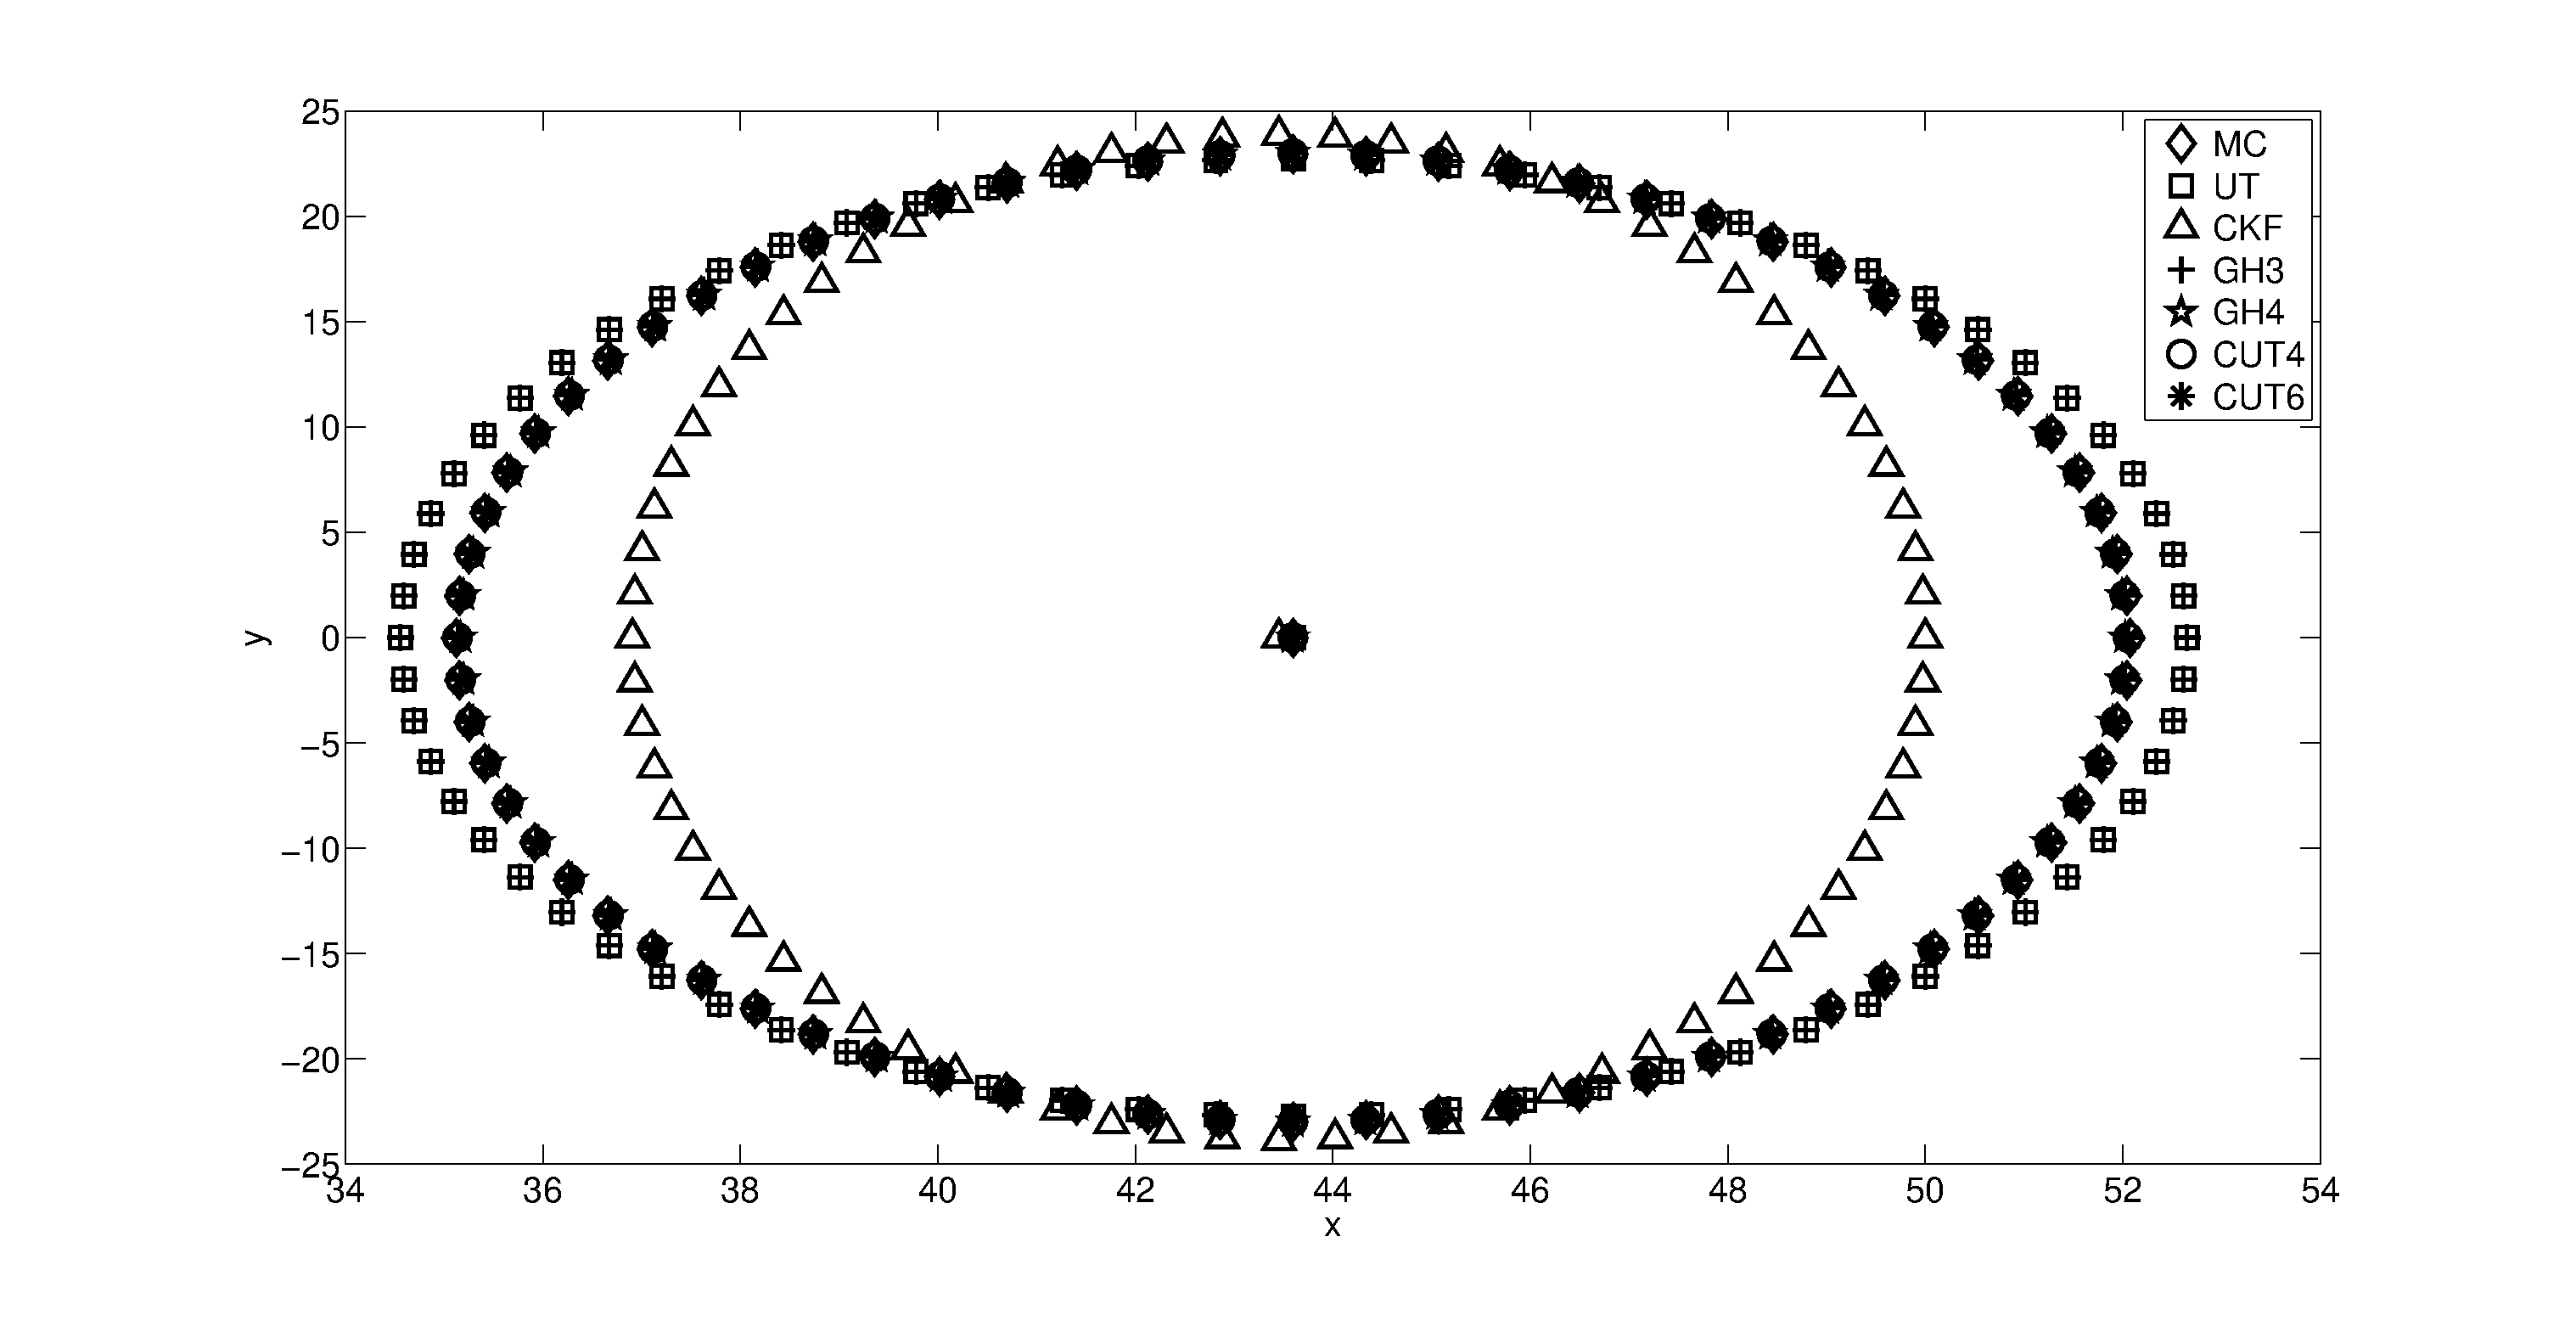
\includegraphics[width=2.7in]{polartocart3}\label{polartocart2}}
      \subfigure[$\mu_r=50$,$\mu_{\theta}=0$,$\sigma_r=0.02^2$,$\sigma_{\theta}=30^2$]{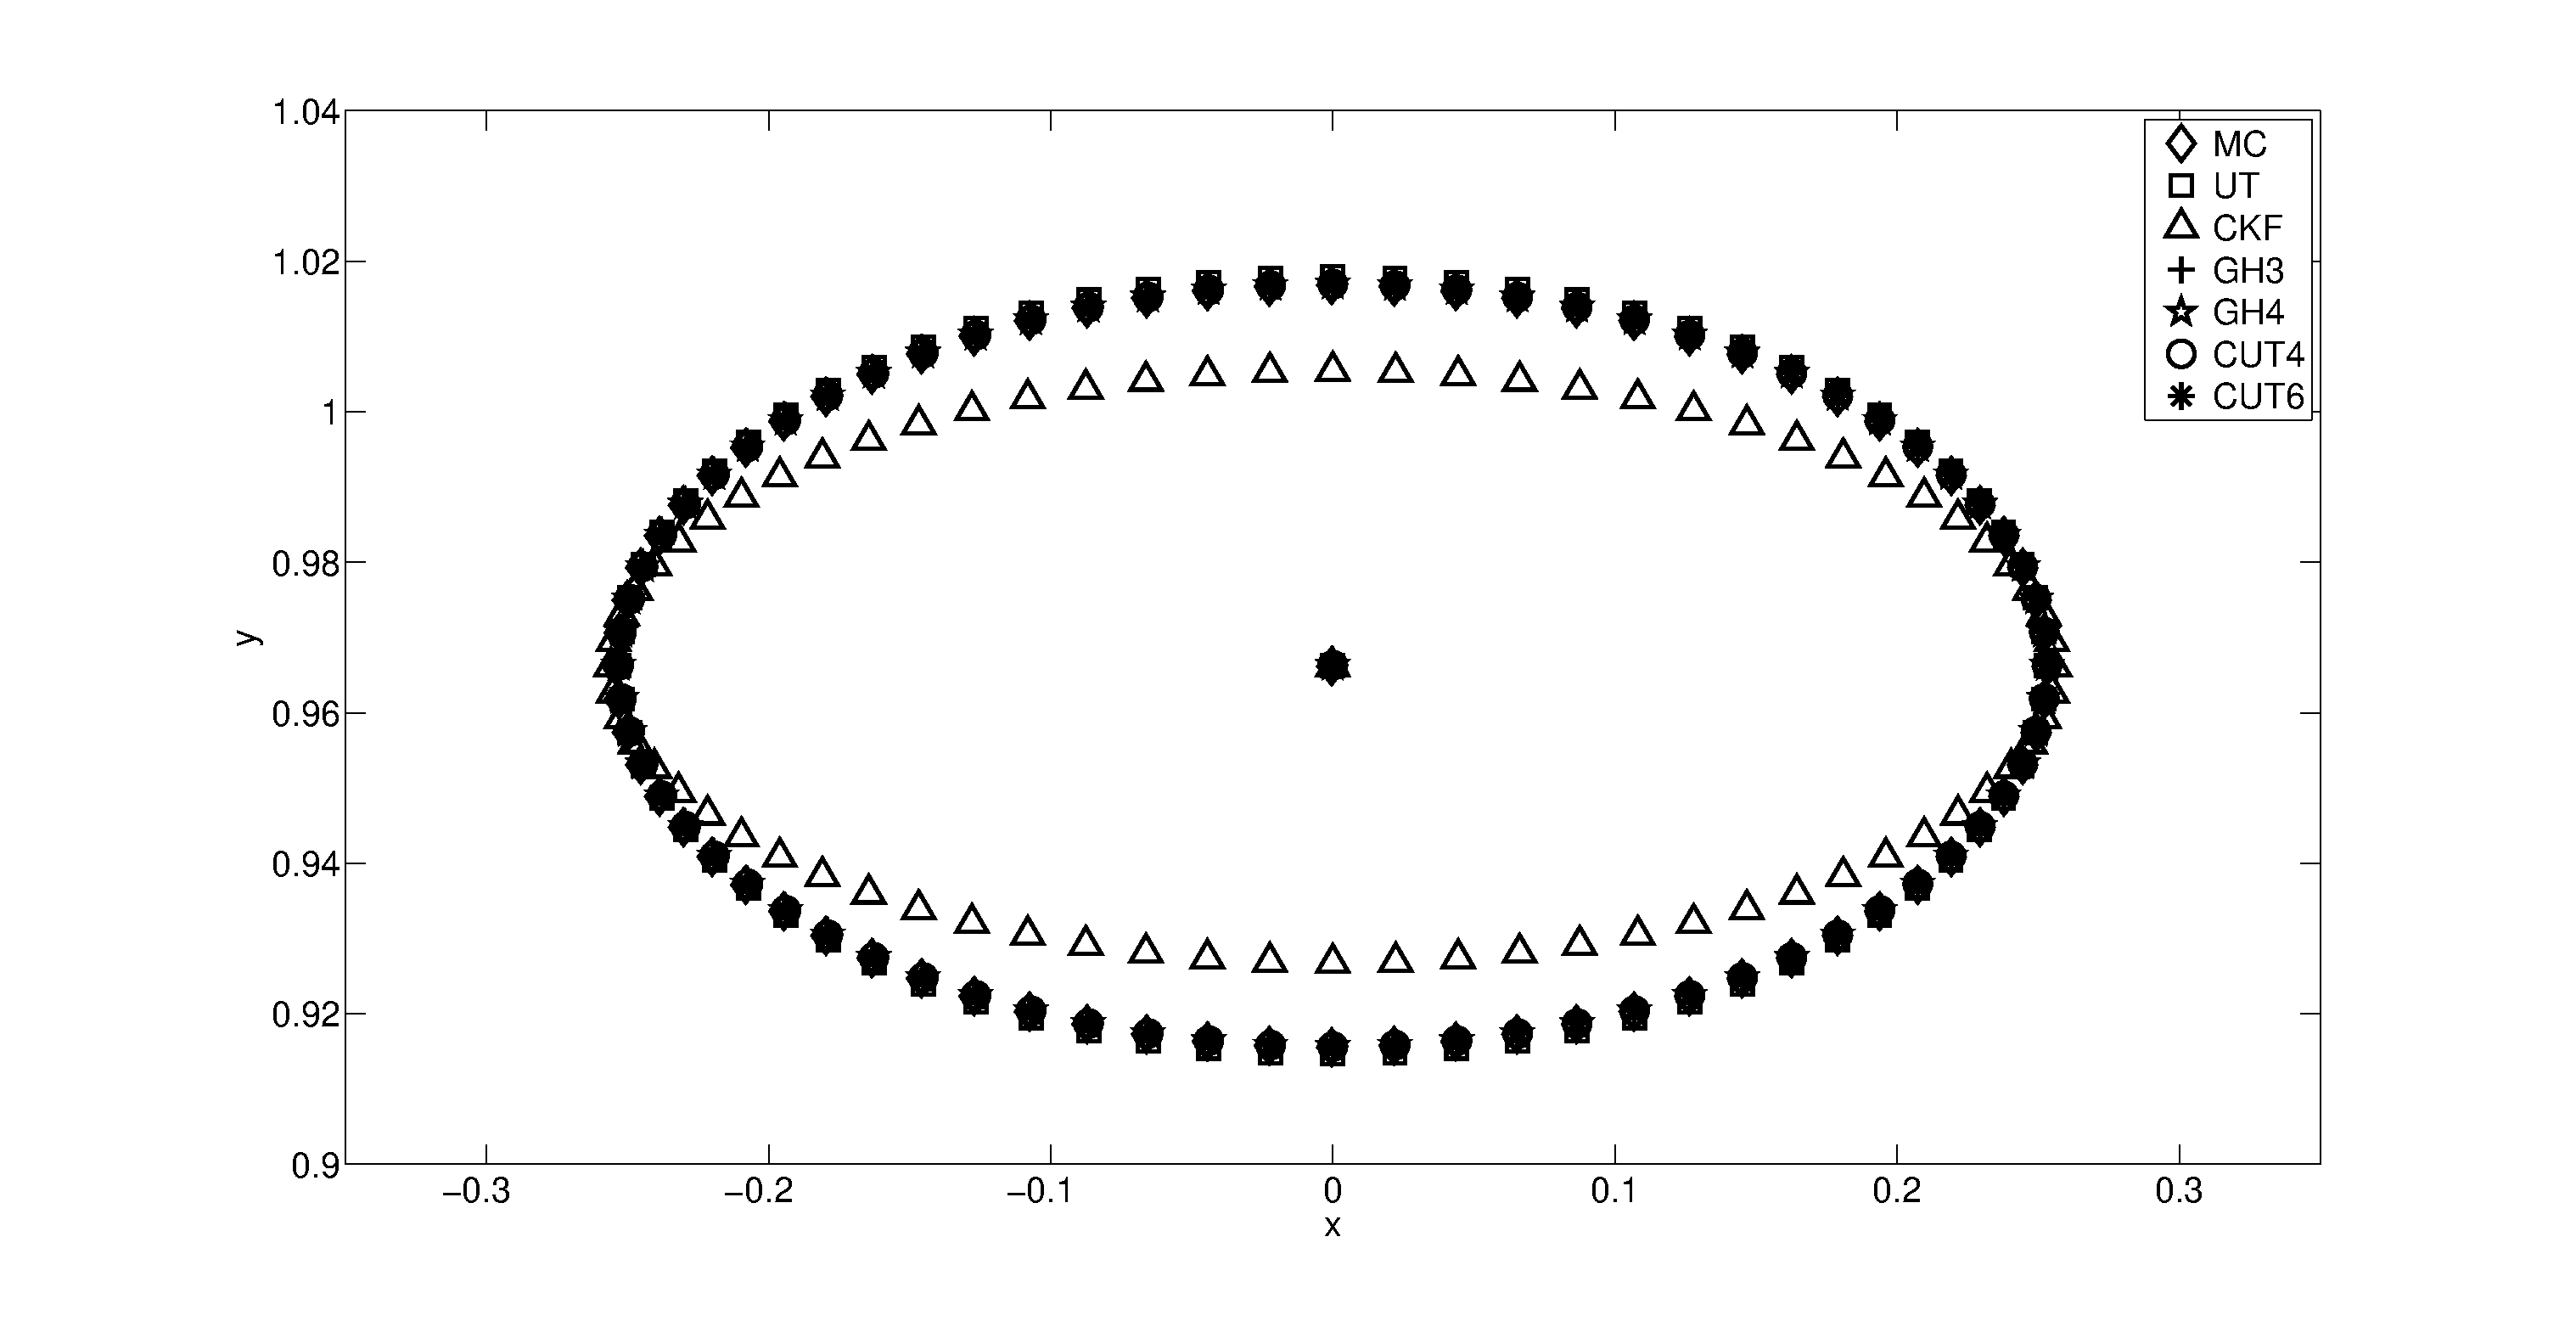
\includegraphics[width=2.6in]{polartocart}\label{polartocart22}}
      \caption{Simulation Results for Polar to Cartesian Transformation. The notations GH2,GH3,GH4$\cdots$ stand for the Gauss Hermite Product rule with 2,3,4$\cdots$ points along each dimension. }
      \label{polartocart4}\vspace{-0.2in}
   \end{figure*} 
   
   
%%%%%%%%%%%%%%%%  Non-polynomial p=-3  %%%%%%%%%%

\subsubsection{$f(\mathbf{X})=(\sqrt{1+\mathbf{X}^T\mathbf{X}})^{\alpha}$, $\mathbf{X}\in\mathbb{R}^N$ } This benchmark problem was introduced in \cite{Arackf}. It has been discussed that computing the expectation of $f(\mathbf{X})$ for negative values for  $\alpha$ is a challenging task since $\alpha<0$  leads to a delta-sequence functions. For simulation purposes, $\alpha=-3$ and the covariance of the zero mean Gaussian pdf is assumed to be 0.1 times the identity matrix.  The covariance is intentionally scaled down by $0.1$ to make the integral value converge with reasonable number of points. Fig.~\ref{pm3gh} shows the relative error with respect to the true value of the expectation integral as a function of GH quadrature points along each dimension while varying the dimension of input space from $2$ to $6$. Fig.~\ref{pm3cut} shows the relative error for dimensions $2$ to $6$ using the CUT methods. Furthermore, Fig.~\ref{pm3ghcutnopts} shows the minimal number of points required for each method to achieve at least $0.5\%$ relative error. It is clear that the proposed CUT8 method yields the accuracy of $0.5\%$ as the GH4 quadrature rule but with a smaller fraction of the number of points. 
%The convergence of the integral is highly effected by increasing the covariance of the normal pdf and is usually characterized by the oscillatory type behaviour of the integral value as a function of number of quadrature points. Even taking a large number of points does not always guarantee the convergence. But by decreasing the magnitude of covariance, most of the quadrature points tend to fall within the region where the function value is significant. Under this condition one can consider the integral value to converge. 
%This example has been shown just to motivate the fact that \textit{as one can capture more moment equations the integral value tends to converge}, this statement is in agreement with equation (\ref{exptinttaylor}).     
\begin{figure*}
   \centering
      \subfigure[Relative Error for GH Quadrature Rule]{\includegraphics[width=2.2in]{gh_methods_err_vs_no_pm3}\label{pm3gh}}
   \subfigure[Relative Error for CUT Method]{\includegraphics[width=2.2in]{cut_methods_err_vs_no_pm3}\label{pm3cut}}
   \subfigure[Minimal Points Required to Achieve $0.5\%$ Relative Error]{\includegraphics[width=2.2in]{no_of_pts_gh4_cut8}\label{pm3ghcutnopts}} 
   \caption{GH vs. CUT: Simulation Results corresponding to $f(\mathbf{X})=(\sqrt{1+\mathbf{X}^T\mathbf{X}})^{-3}$}\vspace{-0.1in}
   \end{figure*}
   
 


\addtolength{\textheight}{-3cm}   % This command serves to balance the column lengths
                                  % on the last page of the document manually. It shortens
                                  % the textheight of the last page by a suitable amount.
                                  % This command does not take effect until the next page
                                  % so it should come on the page before the last. Make
                                  % sure that you do not shorten the textheight too much.

%%%%%%%%%%%%%%%%%%%%%%%%%%%%%%%%%%%%%%%%%%%%%%%%%%%%%%%%%%%%%%%%%%%%%%%%%%%%%%%%

%%%%%%%%%%%%%%%%%%%%%%%%%%%%%%%% CONCLUSIONS %%%%%%%%%%%%%%%%%%%%%%%%%%%%%%%%%%%%%%%%%%%%%%%%
\section{CONCLUSIONS}
 New sets of sigma points are developed to compute multi-dimension expectation integrals involving Gaussian pdf by constraining the points to lie on principal axis and newly define conjugate axis. These new sets of sigma points are guaranteed to exactly reproduce expectation integrals involving polynomial functions up to order 8 with significantly less number of points as compared to the conventional Gaussian quadrature rule. Numerical experiments involving non-polynomial functions are considered to show the efficacy of the developed methodology and numerical results obtained provides a basis for optimism.
 
 
 
% The proposed methodology extends the conventional unscented transformation ideaIt has been customary to use the Guass-Hermite product rule to evaluate multi-dimensional integrals involving the normal probability density function. But the Gauss Hermite product rule not only involves a lot of computational cost but even computational time. Especially for applications in online or real-time filtering, one would prefer a cubature rule with as minimal points as possible without the compromise in accuracy. This has been the prime focus of this paper. Thus we have been able to develop a fully symmetric set of sigma points that are 4th order,  6th order and 8th order equivalent. Developing higher order cubature rules for higher dimensions with minimal points  still remains a challenge. When integrating polynomial functions, each sigma point set can be considered a direct replacement for the equivalent Gauss Hermite product rule of same order.     
%%%%%%%%%%%%%%%%%%%%%%%%%%%%%%%%  ACKNOWLEDGMENTS  %%%%%%%%%%%%%%%%%%%%%%%%%%%%%%%%%%%%%%%%%%%%%%%%
\section{ACKNOWLEDGMENTS}
This material is based upon work supported by the National Science Foundation under Award
No. CMMI- 0908403 and CMMI-1054759.




%%%%%%%%%%%%%%%%%%%%%%%%%%%%%%%%%%%%%%%%%%%%%%%%%%%%%%%%%%%%%%%%%%%%%%%%%%%%%%%%
%\comments{
%\begin{thebibliography}{99}

%\bibitem{c1}
%Stroud A. H., Secrest D, "`Gaussian Quadrature Formulas"',Prentice hall, 1966

%\bibitem{strACMI}
%Stroud A. H., "`Approximate Calculation of Multiple Integrals"', Prentice Hall, 1971

%\bibitem{str2d}
%Stroud A. H.,"'Numerical Integration Formulas of Degree Two"',Mathematics of Computation, Vol. 14, No. 69 (Jan., %1960), pp. 21-26

%\bibitem{phil2D}
%Philip R., Nira R.,"' Perfectly Symmetric Two-Dimensional Integration Formulas with Minimal Numbers of %Points"',Mathematics of Computation, Vol. 23, No. 108 (Oct., 1969), pp. 765-779.

%\bibitem{Robd92D}
%Robert Piessens and Ann Haegemans,"'Cubature Formulas of Degree Nine for Symmetric Planar Regions"',Mathematics of %Computation, Vol. 29, No. 131 (Jul., 1975), pp. 810-815

%\bibitem{Richd72D}
%Richard Franke,"'Minimal Point Cubatures of Precision Seven for Symmetric Planar Regions"',SIAM Journal on Numerical %Analysis, Vol. 10, No. 5 (Oct., 1973), pp. 849-862


%\bibitem{jul1}
%S. J. Julier, J. K. Ulhmann and Whyte,"'A new method for nonlinear transformation of means and covariances in filters %and estimators"', IEEE Trans Automat. Control vol.45, no. 3,pp 472-482 Mar. 2000

%\bibitem{Arackf}
%I Arasaratnam and Simon Haykin,"'Cubature Kalman"',IEEE transactions on Automat. Control, vol 54, no. 6, June 2009

%\bibitem{isser}
%Michalowicz J. V., Nicholas J M,...,"'A general Isserlis theorem for mixed Gaussian random variables "', Statistics %and probability letters...

%\bibitem{dirk}
%SIMON J. JULIER, AND JEFFREY K. UHLMANN,"'Unscented Filtering and Nonlinear Estimation"',PROCEEDINGS OF THE IEEE, VOL. %92, NO. 3, MARCH 2004

%\bibitem{leves}
%A. H. Stroud,"'Some Fifth Degree Integration Formulas for Symmetric Regions"',Mathematics of Computation, Vol. 20, No. %93 (Jan., 1966), pp. 90-97

%\bibitem{jul2}
%A. H. Stroud,"'Some Seventh Degree Integration Formulas for Symmetric Regions"',SIAM Journal on Numerical Analysis, %Vol. 4, No. 1 (Mar., 1967), pp. 37-44


%\end{thebibliography}
%}

%%%%%%%%%%%%%%%%%%%%%%%%% REFERENCES %%%%%%%%%%%%%%%%%%%%%%%%%%%%%%%%%%%%%%%%
\bibliographystyle{IEEEtran}
\bibliography{refcutt}
%%%%%%%%%%%%%%%%%%%%%%%%%%%%%%%%%%%%%%%%%%%%%%%%%%%%%%%%%%%%%%%%%%%%%%%%%%%%%

\end{document}
